\documentclass{template/tp}
\usepackage[utf8x]{inputenc}

\usepackage[frenchb]{babel}
\usepackage[T1]{fontenc}

\usepackage{graphicx}
\usepackage{amssymb}
\usepackage{amsmath}
\usepackage{wasysym} %smiley
\usepackage{hyperref}% hyperliens
\usepackage{tikz}
\usetikzlibrary{babel,positioning,calc}
\usepackage[]{circuitikz}
\usepackage{textcomp}
% \usepackage{minted}
\usepackage[long]{datetime}
\usepackage{gensymb} % \ohm, celsius
\usepackage{framed}
\usepackage{pdfpages}
\usepackage{todo}
\usepackage{paralist}
\usepackage{multicol}

\usepackage{mathastext} % math as standfard text : units are respecting typography conventions.
\usepackage{fancyhdr} %en-tête
\usepackage{qrcode}

% \langexam{frenchb}

\newboolean{koriG}
\ifx\koriG\undefined
\correction{false}
\else
\correction{true}
\fi

\author{Raoul Sommeillier}

%Corrigé ou non?
\correction{false}
% \correction{true}

% Quel TP en pdf output?
%% fancy header & foot
\pagestyle{fancy}
\lhead{[ELEC-H-2001] Électricité\\ TP \no 1 : Circuits résistifs avec sources de tension continue\ifthenelse{\boolean{corrige}}{~-- corrigé}{}}
\rhead{v1.0.1\\ page \thepage}
\cfoot{}
%%

\pdfinfo{
/Author (Raoul Sommeillier, ULB -- BEAMS)
/Title (TP 1 ELEC-H-2001, Circuits résistifs avec sources de tension continue)
/ModDate (D:\pdfdate)
}

\hypersetup{
pdftitle={TP 1 [ELEC-H-2001] Électricité : Circuits résistifs avec sources de tension continue},
pdfauthor={Raoul Sommeillier, ©2018 ULB - BEAMS  },
%pdfsubject={filtrage et analyse fréquentielle}
}

%\date{\vspace{-1cm}\mydate\today}
%\title{\vspace{-2cm} Labo \no 6\\ Électronique appliquée [ELEC-H-301]\\Réalisation d'un ampli à transistor\ifthenelse{\boolean{corrige}}{~\\Corrigé}{}}

%\author{\vspace{-1cm}}%\textsc{Yannick Allard}}

\setlength{\parskip}{0.5cm plus4mm minus3mm} %espacement entre §
\setlength{\parindent}{0pt}


\begin{document}

\tptitle{}{Séance 1~: Circuits résistifs avec sources de tension continue}

\section{Pré-requis}
Avant la séance, vous aurez lu attentivement l'énoncé de la manipulation. Vous aurez par ailleurs relu les chapitres et sections suivants:
\begin{itemize}
	\item Chapitre 1 - Circuits à éléments concentrés
	\begin{itemize}
		\item Section 1.6 - Puissance instantanée, conventions et passivité
	\end{itemize}
	\item Chapitre 5 - Résoudre un circuit : procédure de base et accélérateur
	\begin{itemize}
		\item Section 5.1 -  Vocabulaire lié aux circuits
		\begin{itemize}
			\item 5.1.1 Rappels 
			\item 5.1.2 Connexions série et parallèle
			\item 5.1.3 Branche
			\item 5.1.4 Maille 
		\end{itemize}
		\item Section 5.2 - Lois de Kirchhoff
	\end{itemize}
\end{itemize}

\vspace{5pt}

\newpage

\section{Exercices}
\subsection{Predict-Observe-Explain}
%\ifthenelse{\boolean{assistant}}
%{\color{blue} Exercice prioritaire \\ Timing: 15min \\
%Cet exercice utilise la méthode prédiction-calculs-interprétations des résultats et comparaison des résultats obtenus avec les prédictions.\\ \color{black}}{}
Soit le circuit ci-dessous:
\begin{center}
\begin{circuitikz} \draw
(0,4)   to[battery1, l=$E$, i<=$i$] 	(0,0)
(0,4)--(2,4)--(2,6)
(2,4)   to[R, l=$R_4$, i=$i_2$, v<=$V_2$](7,4)--(8,4)
(2,6)   to[R, l=$R_3$, i=$i_1$]			(7,6)--(7,4)
(8,4)   to[R, l_=$R_1$]					(8,2)
		to[R, l_=$R_2$]					(8,0)--(0,0)		
node[] (A) at (3.5,6) {}
node[] (B) at (5.5,6) {}
(A) to [open, v<=$V_1$] (B)		
node[] (C) at (8.5,4) {}
node[] (D) at (8.5,0) {}
(C) to [open, v^<=$V_3$] (D)
;
\end{circuitikz}
\end{center}

Avec $R_1=R_2=R$, $R_3=2R$ et $R_4=100R$ où $R$ est une valeur de résistance quelconque (différente de $0$)
	
\vspace{10pt}

\Question
{
%question
\textit{Sans résoudre le circuit, pour chaque question (4 questions), entourer la bonne réponse parmi les trois possibilités:}\\
1) \hspace{1cm} $V_2 > V_1$ \hspace{1cm}  $V_2 = V_1$ \hspace{1cm} $V_2 < V_1$\\
2) \hspace{1cm} $V_2 > V_3$ \hspace{1cm}  $V_2 = V_3$ \hspace{1cm} $V_2 < V_3$\\
3) \hspace{1cm}  $i_1 > i_2$ \hspace{1.25cm}  $i_1 = i_2$ \hspace{1.25cm} $i_1 < i_2$\\
4) \hspace{1cm} $i > i_2$ \hspace{1.4cm}  $i = i_2$ \hspace{1.4cm} $i < i_2$\\
}
{%correction
\textbf{$V_2 = V_1$},
\textbf{$V_2 < V_3$},
\textbf{$i_1 > i_2$}, et 
\textbf{$i > i_2$}.
\begin{itemize}
\item Le but de cet exercice est de vous permettre de vérifier si votre intuition est un bon guide... ou vous induit plutôt en erreur (et sur quoi précisément). Il est donc important d'essayer de trouver les réponses sans résoudre explicitement le circuit, et de comparer avec la résolution ensuite.
\item 1) $V_1$ et $V_2$ sont en parallèle, donc leurs ddps sont identiques
\item 2) A première vue, on peut être tenté de pense que $V_2>V_3$ car $R_4$ (sur laquelle est prise $V_2$) est $>(R_1+R_2)$. C'est oublier qu'il y a une résistance $R_3$ en parallèle sur $R_4$, et que la majorité du courant passera dans $R_3$. Le courant dans $R_4$ et dans $R_1/R_2$ ne sont pas du tout les mêmes.
\item 3) car $R_3<<R_4$
\item 4) $i$ est la somme de $i_1$ et $i_2$ qui sont tous les deux positifs
\item ... voir confirmations par calcul rigoureux ci-dessous
\end{itemize}
}
%{%assistant
%On s’attend à ce que l’étudiant pense que le fait d’avoir une grande résistance $R_4$ diminue fortement le courant délivré par la source, négligeant l’influence de $R_3$ de faible valeur par rapport à $R_4$. La notion d’équipotentielle est abordée (via $V_2=V_3$ mais dont la longueur des flèches peut induire l’étudiant en erreur) et la connaissance « qualitative » de la loi des nœuds est vérifiée.  
%}

\Question
{%Question
\textit{Calculer le courant $i$ délivré par la source ainsi que les courants $i_1$ et $i_2$, et les tensions $V_2$ et $V_3$.}
}
{%Corrigé
$i_{source}=\frac{E}{R_{éq}}$\\
$R_{éq}=R_1+R_2+\frac{R_3 R_4}{R_3+R_4}=2R+\frac{200R}{102}=(2+\frac{200}{102})R=3,96R$\\
$V_3=(R_1+R_2)i=\frac{2E}{2+\frac{200}{102}}=0,505E$\\
$V_2=E-V_3=E(1-\frac{2}{2+\frac{200}{102}})=0,495E$\\
$V_1=V_2$\\
$i_1=\frac{V_2}{R_3}=\frac{E}{R_3}(1-\frac{2}{2+\frac{200}{102}})=\frac{E}{2R}(1-\frac{2}{2+\frac{200}{102}})$\\
$i_2=i-i_1=\frac{V_2}{R_4}=\frac{E}{R_4}(1-\frac{2}{2+\frac{200}{102}})=\frac{E}{100R}(1-\frac{2}{2+\frac{200}{102}})=\frac{i_1}{50}$
}
{%Assistant
%/
%}

\Question
{%Question
\textit{Comparer les résultats obtenus avec vos réponses aux questions précédentes.}
}
{%Corrigé
La présence de grandes résistances dans un circuit n'est pas synonyme d'un petit courant fourni par la source. En effet, la résistance $R_4$ est très élevée mais la résistance $R_3$, placée en parallèle avec $R_4$, permet le passage de la majorité d'un courant important provenant de la source. Le courant $i_2$ est bien moins important que le courant $i_1$ (facteur $50$).
}
%{%Assistant
%L’étudiant doit comparer ses prédictions à ses résultats et en déduire, sans qu’on lui dise, que la présence de grandes résistances n’est pas synonyme d’un petit courant fourni par la source.
%}

\subsection{Predict-Observe-Explain 2}
%\ifthenelse{\boolean{assistant}}
%{\color{blue} Exercice prioritaire \\ Timing: 10min \\
%
%Le but est de déstabiliser l’étudiant avec une configuration de fils peu commune. Il doit, seul, pouvoir identifier la configuration simple des deux circuits (mise en parallèle). La notion d’équipotentielle des fils est exploitée. L’exercice exploite la méthode prédiction-calculs-interprétations des résultats et comparaison des résultats obtenus avec les prédictions.\\ \color{black}}{}

Considérer les deux circuits suivants:
%\begin{multicols*}{2} 
\begin{center}
\begin{circuitikz} \draw
(0,0)   -- (0,3) -- (1,3)
(1,2)   -- (1,4)
(1,2)   to[R, *-*, l=$R$] (5,2)
(1,2)   to[R, l=$R$] (5,4)
(1,4)   to[R, *-*, l=$R$] (5,4)--(5,2)
(5,3)--(6,3)--(6,0)
(0,0)		to[battery1, l_=$E$, i_=$i_a$] (6,0)
(3,5.5) node[]{Circuit a}
;
\end{circuitikz}
\hspace{1cm}
%\end{center}
%\newpage 
%\begin{center}
\begin{circuitikz} \draw
(0,0)   -- (0,3) -- (1,3)
(1,2)   -- (1,4)
(1,2)   to[R, *-*, l=$R$] (5,2)
(1,2)   to[R, l=$R$] (5,4)
(1,4)   to[R, *-*, l=$R$] (5,4)--(5,2)
(1,4)   to[R, l_=$R$] (3,3)--(5,2)
(5,3)--(6,3)--(6,0)
(0,0)		to[battery1, l_=$E$, i_=$i_b$] (6,0)
(3,5.5) node[]{Circuit b}
;
\end{circuitikz}
\end{center}
%\end{multicols*}

\Question
{%Question
\textit{Sans résoudre les circuits, lequel des deux verra apparaître le courant le plus important fourni par la source?}
}
{%Corrigé
Le circuit $b$. L’ajout d’une résistance ne mène pas toujours à une diminution du courant fourni par la source. Dans les deux circuits $a$ et $b$, les résistances sont toutes placées en parallèle. Cependant, le circuit $a$ en compte 3 alors que le circuit $b$ en compte 4.
}
%{%Assistant
%On s’attend à ce que l’étudiant réponde que le circuit où le plus grand nombre de résistances se trouve mènera à un courant délivré par la source moins important. On vise donc à détruire la préconception selon laquelle l’ajout d’une résistance mène toujours à une diminution du courant fourni par la source.
%}

\Question
{%Question
\textit{Calculer le courant fourni par la source pour chaque circuit.}
}
{%Corrigé
Simplifier le circuit: les schémas $a$ et $b$ de départ son d'une configuration inutilement complexe, graphiquement parlant. Il vaut mieux réécrire le circuit selon les schémas suivants:
\begin{center}
\begin{circuitikz} \draw
(0,0)   -- (0,3) -- (1,3)
(1,2)   -- (1,4)
(1,2)   to[R, *-*, l=$R$] (5,2)
(1,3)   to[R, *-*, l=$R$] (5,3)
(1,4)   to[R, *-*, l=$R$] (5,4)--(5,2)
(5,3)--(6,3)--(6,0)
(0,0)		to[battery1, l_=$E$, i_=$i_a$] (6,0)
(3,5.5) node[]{Circuit a}
;
\end{circuitikz}
\hspace{1cm}
%\end{center}
%\newpage 
%\begin{center}
\begin{circuitikz} \draw
(0,0)   -- (0,3) -- (1,3)
(1,2)   -- (1,4)
(1,2)   to[R, *-*, l_=$R$] (5,2)
(1,3.5)   to[R, *-*] (5,3.5)
(1,4)   to[R, *-*, l=$R$] (5,4)--(5,2)
(1,2.5)   to[R, *-*, l=$R$] (5,2.5)
(5,3)--(6,3)--(6,0)
(0,0)		to[battery1, l_=$E$, i_=$i_b$] (6,0)
(3,5.5) node[]{Circuit b}
;
\end{circuitikz}
\end{center}
Le courant fourni par la source du circuit $a$ est $\frac{3E}{R}$.\\
Le courant fourni par la source du circuit $b$ est $\frac{4E}{R}$.\\
Le courant fourni par la source du circuit $a$ est donc inférieur au courant fourni par la source du circuit $b$.\\
}
%{%Assistant
%/
%}

\Question
{%Question
\textit{La disposition des éléments dans les deux circuits simplifie-t-elle la résolution des circuits?}
}
{%Corrigé
Il est utile de simplifier le circuit avant de le résoudre pour se concentrer sur l'objectif de la question. Comme dans l'exercice précédent, l'ajout d'une résistance dans un circuit n'entraîne pas systématiquement une augmentation de la résistance totale équivalente vue depuis le source. En effet, ici, le circuit $b$ contient plus de résistances (en nombre d'éléments) mais conduit à une résistance équivalente plus faible du point de vue de la source, menant à un courant tiré de la source plus élevé que dans le cas du circuit $a$.
}
%{%Assistant
%L’étudiant doit conclure de cet exercice qu’il est primordial de simplifier le circuit avant de le résoudre, tant en calculant des résistances équivalentes qu’en réécrivant proprement le circuit de manière à avoir des fils posés proprement (proprement = tous les fils sont parallèles ou à 90° entre eux, mais pas à 45° comme dans les deux circuits présentés). Il doit également conclure que l’ajout d’une résistance peut mener à un courant délivré par la source plus important.
%}

%\ifthenelse{\boolean{corrige}}{\newpage}{}
\subsection{Démonstration 1}
%\ifthenelse{\boolean{assistant}}
%{\color{blue} Exercice prioritaire \\ Timing: 15min \\ \color{black}}{}
Pour le circuit ci-dessous:
\begin{center}
\begin{circuitikz} \draw
(0,0)   -- (0,3) -- (1,3)
(1,2)   -- (1,4)
(1,2)   to[R, *-*, l=$R_3$] (3,2) to[R, *-*, l=$R_4$] (5,2)
(1,4)   to[R, *-*, l=$R_1$] (3,4) to[R, *-*, l=$R_2$] (5,4)--(5,2)
(5,3)--(6,3)--(6,0)
(0,0)		to[battery1, l_=$E$, i_=$i$] (6,0)
(3,2)--(3,4)
(3.3,3) node[]{(1)}
;
\end{circuitikz}
\end{center}

La connexion verticale (1) est une équipotentielle et ne peut donc pas être parcourue par un courant. En effet, la loi d’Ohm renseigne que V=RI, ce qui implique que s’il n’y a pas de chute de potentiel, il n’y a pas de courant. Comme il n’y a pas de courant, le circuit précédent est équivalent à celui-ci :
\begin{center}
\begin{circuitikz} \draw
(0,0)   -- (0,3) -- (1,3)
(1,2)   -- (1,4)
(1,2)   to[R, *-*, l=$R_3$] (3,2) to[R, *-*, l=$R_4$] (5,2)
(1,4)   to[R, *-*, l=$R_1$] (3,4) to[R, *-*, l=$R_2$] (5,4)--(5,2)
(5,3)--(6,3)--(6,0)
(0,0)		to[battery1, l_=$E$, i_=$i$] (6,0)
;
\end{circuitikz}
\end{center}
Étant donné que $R1$ est en série avec $R2$ et que $R3$ est en série avec $R4$, et que ces deux groupes ($R1+R2$) et ($R3+R4$) sont en parallèle, on déduit que le courant $i$ fourni par la source $E$ vaut:
$$i=\frac{E}{\frac{(R_1+R_2)(R_3+R_4)}{R_1+R_2+R_3+R_4}}$$

\Question
{%Question
\textit{Démontrer que ce raisonnement est erroné.}
}
{%Corrigé
La connexion verticale ne peut pas de tout être supprimée car elle est parcourue (en tout cas, elle peut l'être) par un courant. La loi d'Ohm $V=RI$ peut être appliquée, mais dans celle-ci $R=0$ et $V=0$, de sorte que $i$ peut être non nul.\\
N.B.: Si l'on prend le cas où toutes les résistances sont égales, pensez-vous qu'on puisse supprimer le fil (1)?
}
%{%Assistant
%L’exercice se base sur une fausse démonstration. Elle fait appel à des résultats que l’étudiant devrait juger corrects. Il est essentiel que l’étudiant vérifie chacune des informations fournies dans la fausse démonstration –encouragez la discussion entre étudiants. On s’attend, entre autres, que l’étudiant vérifie de nombreuses fois la formule du i en fin de démonstration, ce qui lui permettra par la même occasion de s’approprier les deux formules de mise en série et en parallèle de résistances. La loi d’Ohm est très connue par les étudiants, et on s’attend à ce qu’ils l’utilisent hors de son domaine de validité.
%}

\subsection{Simplification}
%\ifthenelse{\boolean{assistant}}
%{\color{blue} Exercice non prioritaire \\ Timing: 10min \\
%L’exercice vise à déstabiliser l’étudiant car ce circuit sera (sans doute) visuellement plus complexe que tous les circuits qu’il aura vus jusqu’ici. Il sera déstabilisé et sera donc poussé à reconnaître qu’il a des connaissances et compétences à mobiliser pour improviser correctement. On s’attaque à la préconception selon laquelle tous les éléments électriques sont soit en parallèle soit en série.\\ \color{black}}{}
\Question
{%Question
\textit{Deux types de configuration de résistances ont été vus en BA1: les résistances en série et les résistances en parallèle. Pourquoi ces notions sont-elles utiles pour résoudre un circuit électrique?}
}
{%Corrigé
La notion de résistance équivalente série et parallèle est utile pour simplifier un schéma afin de calculer plus efficacement les grandeurs recherchées. Il est néanmoins important de se rendre compte que deux résistances connectées peuvent n'être ni en série ni en parallèle.
}
%{%Assistant
%/
%}

Dans le circuit suivant, où toutes les sources sont égales à $E$ et toutes les résistances à $R$,
\begin{center}
\begin{circuitikz} \draw
(0,6)   to[battery1] (0,4) to[battery1] (0,2) to[battery1] (0,0)
(0,6)--(2,6)--(2,4)
(0,0)--(2,0)to[R] (2,4)to[R] (4,4) to[R](6,4)
(2,0)to[R](4,0)to[R](4,4)
(2,6)to[R](6,6)--(6,4)to[R](8,4)to[R](10,4)to[R](12,4)
(4,0)to[R](10,0)to[R](14,0)--(14,6)to[R](12,6)--(12,4)to[R](14,4)
(6,6)to[R](8,6)--(8,4)
;
\end{circuitikz}
\end{center}
\Question
{%Question
\textit{Identifier les parties de circuit qui peuvent être redessinées en utilisant les notions de configurations en parallèle et en série. Dessiner le schéma simplifié qui en résulte.}
}
{%Corrigé
Les résistances encadrées sont en série, et celles entourées sont en parallèle:
\begin{center}
\begin{circuitikz}[scale=0.8] \draw
(0,6)   to[battery1] (0,4) to[battery1] (0,2) to[battery1] (0,0)
(0,6)--(2,6)--(2,4)
(0,0)--(2,0)to[R] (2,4)to[R] (4,4) to[R](6,4)
(2,0)to[R](4,0)to[R](4,4)
(2,6)to[R](6,6)--(6,4)to[R](8,4)to[R](10,4)to[R](12,4)
(4,0)to[R](10,0)to[R](14,0)--(14,6)to[R](12,6)--(12,4)to[R](14,4)
(6,6)to[R](8,6)--(8,4)
;
\draw[dashed] (8.2,3.5) -- (8.2,4.5)--(11.8, 4.5)--(11.8,3.5)--(8.2,3.5);
\draw[dashed] (5.2,-0.5) -- (5.2,0.5)--(13.8, 0.5)--(13.8,-0.5)--(5.2,-0.5);
\draw[dashed] (7,5)circle(1.3);
\draw[dashed] (13,5)circle(1.3);
\end{circuitikz}
\end{center}

Il en résulte le schéma suivant, où 4 résistances sont encore en série et où la source de tension équivalente a été calculée (trois fois la même source de tension en série):
\begin{center}
\begin{circuitikz}[scale=0.8] \draw
(0,0)   to[battery1, l=$3E$, invert](0,6)--(2,6)--(2,4)
(0,0)--(2,0)to[R] (2,4)to[R] (4,4) to[R](6,4)
(2,0)to[R](4,0)to[R](4,4)
(2,6)to[R](6,6)--(6,4)to[R, l=$R/2$](8,4)to[R, l=$2R$](12,4)
(4,0)to[R, l=$2R$](14,0)--(14,4)to[R, l=$R/2$](12,4)
;
\draw[dashed] (6.2,-0.5) -- (6.2,5)--(14.2, 5)--(14.2,-0.5)--(6.2,-0.5);
\end{circuitikz}
\end{center}
Ce schéma peut alors encore être simplifié étant donné la présence de 4 résistances en série encadrées. Il en résulte le schéma suivant:
\begin{center}
\begin{circuitikz}[scale=0.8] \draw
(0,0)   to[battery1, l=$3E$, invert](0,6)--(2,6)--(2,4)
(0,0)--(2,0)to[R] (2,4)to[R] (4,4) to[R](6,4)
(2,0)to[R](4,0)to[R](4,4)
(2,6)to[R](6,6)--(6,4)to[R, l=$5R$](6,0)--(4,0)
;
\end{circuitikz}
\end{center}

}
%{%Assistant
%/
%}



\textit{Il est impossible de réduire le schéma précédent à celui-ci:}
\begin{center}
\begin{circuitikz} \draw
(0,0)   to[battery1, l=$E_{totale_{\acute{e}quivalente}}$, invert] (0,3)--(2,3)
(0,0)--(2,0) to[R, l_=$R_{totale_{\acute{e}quivalente}}$] (2,3)
;
\end{circuitikz}
\end{center}
\Question
{%Question
\textit{Expliquer pourquoi cette affirmation (écrite en italique) est incorrecte.}
}
{%Corrigé
Dans le dernier schéma redessiné, il reste des résistances qui ne sont ni en série, ni en parallèle. Ceci n'empêche pas de trouver par calcul une valeur de résistance équivalente, qui est simplement la ddp de la source divisée par le courant fourni par la source: $\frac{E_{totale_{\acute{e}quivalente}}}{I_{totale_{\acute{e}quivalente}}}=\frac{3E}{I_{totale_{\acute{e}quivalente}}}$.
}
%{%Assistant
%L’étudiant devrait alors comprendre que calculer le rapport Etotal/itotal permet de calculer une résistance équivalente, après avoir résolu le circuit entièrement. Il doit déduire que la préconception traitée n’est pas correcte (tous les éléments sont soit en série, soit en parallèle).
%}

\subsection{Démonstration 2}
%\ifthenelse{\boolean{assistant}}
%{\color{blue} Exercice prioritaire \\ Timing: 15min \\ \color{black}}{}
Pour le schéma suivant, avec $R=100 \Omega$, $E_1=100V$ et $E_2=50V$,
\begin{center}
\begin{circuitikz} \draw
(0,3)   to[battery1, v_<=$E_1$, i<=$i$] (0,0)
(0,3)--(1,3)to[R, l=$R$, v>=$V_R$](3,3)--(4,3)
(0,0)--(4,0) to[battery1, v_>=$E_2$,invert] (4,3)
;
\end{circuitikz}
\end{center}
Comme les tensions $E_1$ et $E_2$ sont de polarité opposée, en utilisant la loi des mailles, nous trouvons que $E_1 + V_R = E_2$.\\

De ceci, nous déduisons, puisque $V_R=Ri$, $i =-0,5A$\\

La puissance liée à la source $E_1$ vaut donc $p(E_1)=i*E_1 = -0,5 A * 100 V = -50 W$.\\
Étant donné que cette puissance est négative, nous en déduisons que $E_1$ agit comme une charge. En effet, pour une puissance positive, une source fournit de l'énergie au circuit (typiquement, la batterie se décharge), alors que pour une puissance négative, la source consomme de l'énergie du circuit (typiquement, la batterie est chargée). Comme l'énergie ne peut pas venir de nulle part, nous en déduisons que $E_2$ est une source.\\

Cependant, selon le circuit suivant :
\begin{center}
\begin{circuitikz} \draw
(0,3)   to[battery1, v_<=$E_1$, i<=$i$] (0,0)
(0,3)--(1,3)to[R, l=$R$, v<=$V_R$](3,3)--(4,3)
(0,0)--(4,0) to[battery1, v_>=$E_2$,invert] (4,3)
;
\end{circuitikz}
\end{center}
L’équation de maille devient : $E_1 = V_R + E_2$ menant à un courant $i=+0,5A$. Nous en déduisons que la puissance associée à la source $E_1$ vaut $p(E_1)= i*E_1 = +0,5A * 100 V = 50W$.\\
Comme la puissance est positive, la source $E_1$ est une source. Nous en déduisons que $E_2$ agit comme une charge pour respecter le principe de conservation de l'énergie.
\Question
{%Question
\textit{Comment peut-on expliquer cette contradiction ? }
}
{%Corrigé
Cet exercice se base sur le principe de la fausse démonstration. Il met l'accent sur l'importance des conventions de signes et de flèches associés aux grandeurs électriques. Les conventions générateur/récepteur devraient ressortir comme étant indispensables.\\

Dans les deux cas, les lois des mailles sont correctement écrites. Par contre, pour le premier schéma, on doit écrire, vu les sens des tensions et courants choisis, $V_R=-RI$, ce qui donne $i=+0,5A$ et donc la même réponse que pour le second schéma.\\

En effet: pour une résistance, en écrivant la loi constitutive, si la tension est définie dans le sens opposé du courant, la loi est $V=RI$. Si la tension est définie dans le même sens que le courant, la loi est $V=-RI$. On ne peut donc pas écrire la loi $V=RI$ sans faire attention au sens du courant et de la tension utilisés (et à fortiori si on n'a défini aucun sens!). L'utilisation systématique des conventions générateur et récepteur permet justement d'éviter de faire des erreurs de ce type.
}
%{%Assistant
%Cet exercice se base sur le principe de la fausse démonstration. Il met l’accent sur l’importance des conventions de signes et de flèches associés aux grandeurs électriques. Les conventions générateur/récepteur devraient ressortir comme étant indispensables par l’étudiant, pour faute de pouvoir démontrer un résultat qui n’est pas correct. L’étudiant devrait être perturbé par ceci : il/elle a l’habitude de voir que les flèches associées à la tension de la charge et de la source pour un simple circuit « 1 source, 1 résistance », doivent être opposés. On exploite cette idée là dans cet exercice. Les résultats paraîtront logiques à l’étudiant. Posez des questions aux étudiants pour favoriser la discussion entre eux et avec vous, mais n’indiquez pas l’endroit où la démonstration utilise des résultats erronés.
%}

\subsection{Du circuit aux équations}
%\ifthenelse{\boolean{assistant}}
%{\color{blue} Exercice non prioritaire \\ Timing: 10min \\ \color{black}}{}
Soit le circuit suivant:
\begin{center}
\begin{circuitikz} \draw
(0,0)   to[battery1, v=$10V$, invert] (0,2)to[R, l=$3\Omega$](4,5)to[battery1,v=$20V$, invert](10,5)
(0,0)--(10,0)to[battery1,v=$5V$, invert](10,2)to[R,l=$3\Omega$](10,4)--(10,5)
(0,2) to[R,l=$3\Omega$](6,3)to[R,l=$3\Omega$](10,4)
(6,0)to[R,l=$3\Omega$](6,1.5)to[battery1,v=$30V$, invert](6,3)
;
\end{circuitikz}
\vspace{1cm}
\end{center}
\Question
{%Question
\textit{Écrire les équations de Kirchhoff de ce circuit. Indiquer quelles sont les charges et quelles sont les sources selon les conventions utilisées. Ne pas résoudre les équations.}
}
{%Corrigé
Simplifiez d'abord le circuit visuellement parlant. On arrive au schéma de gauche:
\begin{center}
\begin{circuitikz} \draw
(0,0)--(0,2)   to[battery1, v=$10V$, invert] (0,4)to[R, l=$3\Omega$](2,4)
(2,0)to[R, l=$3\Omega$](2,2)   to[battery1, v=$30V$, invert] (2,4)to[R, l=$3\Omega$](4,4)
(4,0)to[R, l=$3\Omega$](4,2)   to[battery1, v=$5V$, invert] (4,4)--(4,6)
(0,0)--(4,0)
(0,4)--(0,6)to[R, l=$3\Omega$](2,6)   to[battery1, v=$20V$, invert] (4,6)
;
\end{circuitikz}
%\end{center}
%\begin{center}
\begin{circuitikz} \draw
(0,0)--(0,2)   to[battery1, v=$E_1$, i>=$i_1$, invert] (0,4)to[R, v<=$V_{R_5}$, i=$i_5$](2,4)
(2,0)to[R, v<=$V_{R_2}$](2,2)   to[battery1, v=$E_2$, i>=$i_2$, invert] (2,4)to[R, v<=$V_{R_6}$, i=$i_6$](4,4)
(4,0)to[R, v<=$V_{R_5}$](4,2)   to[battery1, v=$E_3$, i>=$i_3$, invert] (4,4)--(4,6)
(0,0)--(4,0)
(0,4)--(0,6)to[R, v<=$V_{R_4}$, invert](2,6)   to[battery1, v=$E_4$, i>=$i_4$, invert] (4,6)
;
\end{circuitikz}
\end{center}

Ensuite, il faut définir les tensions et les courants (schéma de droite)\\
En respectant les conventions récepteur-générateur systématiquement: on définit tous les courants puis on définit les tensions dans le même sens pour l'élément source, et dans le sens opposé pour l'élément résistance.\\
Conseil: éviter d'utiliser les valeurs numériques lors de l'écriture d'équations. Même si toutes les valeurs sont fournies directement, nommer les éléments $E_1$, $E_2$,... $R_1$, $R_2$,... pour éviter une source d'erreurs de distraction.

Les 3 équations de mailles sont:
$$E_1-V_{R_5}-E_2+V_{R_2}=0$$
$$E_2-V_{R_6}-E_3+V_{R_3}-V_{R_2}=0$$
$$E_4+V_{R_6}+V_{R_5}-V_{R_4}$$

Les équations de nœuds sont (3 suffisent):
$$i_1-i_4-i_5=0$$
$$i_5+i_2-i_6=0$$
$$i_4+i_6+i_3=0$$
$$-i_1-i_2-i_3=0$$

Et les équations constitutives sont $V_{R_k}=R_k I_k$ pour $k=2,3...,6$ car le courant a toujours un sens choisi opposé à celui de la tension sur le schéma ci-dessus.\\

Souvent, la tension associée à une source continue sera caractérisée par une flèche allant de la borne négative à la borne positive. Dans les deux schémas ci-dessus, cette habitude à été suivie.
}
%{%Assistant
%L’exercice a pour but de déstabiliser les étudiants par une mauvaise représentation des éléments (éléments formant des angles aléatoires entre eux) et de les driller à définir les tensions et courants des éléments suivant une convention. Cela illustre les premières étapes fondamentales pour la résolution d’un circuit électrique (définir i et v et respect des conventions, simplifications (réécriture du circuit, R équivalentes…), poser les équations).
%}

\Question
{%Question
\textit{Comparer les sens définis par un de vos voisins. Cela influence-t-il le résultat ?}
}
{%Corrigé
Le résultat final (c'est-à-dire, les tensions et courants associés aux différents éléments, compte tenu des sens choisis) ne change pas, quels que soient les sens associés aux différents éléments.
}
%{%Assistant
%Cette sous question a pour but de mettre en avant la liberté des étudiants quant aux sens associés aux courants en particulier. Un étudiant pourrait respecter une convention générateur (i et v de même sens) pour la source de 30 V et un autre pourrait lui associer une convention récepteur (i et v de sens opposés). L’étudiant devrait prendre également conscience du fait que changer le sens de la flèche associée un V ou i permet de changer le signe de la grandeur décrite. Ils devraient comprendre que la physique du problème ne changera pas si les résultats sont bien interprétés avec les conventions choisies.
%}

\subsection{Résolution d'un circuit}
%\ifthenelse{\boolean{assistant}}
%{\color{blue} Exercice non prioritaire \\ Timing: 10min \\
%Le but de la séance est de pouvoir résoudre tout circuit résistif avec sources de tension continue, ce qui est résumé dans cet exercice. Il demande à l’étudiant de respecter la stratégie vue au cours pour résoudre un circuit. Les étudiants devront également donner des noms aux éléments sans qu’on leurs les fournisse.\\ \color{black}}{}
\Question
{%Question
\textit{Écrire votre démarche de résolution de circuits en phrases.}
}
{%Corrigé
Cfr slides du cours
}
%{%Assistant
%/
%}

Soit le circuit suivant où toutes les sources se le SMS a bien été envoyé par le numéro de téléphone rattaché au comptont égales à $10V$ et toutes les résistances à $10\Omega$:
\begin{center}
\begin{circuitikz} \draw
(0,0)   to[battery1, invert] (0,4)to[R](4,4)--(8,4)--(8,3)
(0,0)--(8,0)--(8,1)
(4,4) to[battery1, invert](4,2)to[R](4,0)
(7,3)--(9,3)
(7,1)--(9,1)
(7,1)to[R](7,3)
(9,1)to[R](9,3)
;
\end{circuitikz}
\end{center}
\Question
{%Question
\textit{Trouver tous les courants et toutes les tensions de ce circuit (sources comprises).}
}
{%Corrigé
\begin{center}
\begin{circuitikz} \draw
(0,0)   to[battery1, v=$E_1$, i>=$i_1$, invert] (0,4)to[R, l=$R_1$,v<=$V_{R_1}$](4,4)to[short, i=$i_3$](8,4)--(8,3)
(0,0)--(8,0)--(8,1)
(4,4) to[battery1, v=$E_2$, i>=$i_2$, invert](4,2)to[R, l=$R_2$,v<=$V_{R_2}$](4,0)
(7,3)--(9,3)
(7,1)--(9,1)
(7,1)to[R, l=$R_3$, v>=$V_{R_3}$, i<^=$i_4'$](7,3)
(9,1)to[R, l=$R_4$, v>=$V_{R_4}$, i<^=$i_4$](9,3)
;
\end{circuitikz}
\end{center}

$V_{R_4}=V_{R_3}$ et on transforme le schéma en:
\begin{center}
\begin{circuitikz} \draw
(0,0)   to[battery1, v=$E_1$, i>=$i_1$, invert] (0,4)to[R, l=$R_1$,v<=$V_{R_1}$](4,4)to[short, i=$i_3$](8,4)--(8,3)
(0,0)--(8,0)--(8,1)
(4,4) to[battery1, v=$E_2$, i>=$i_2$, invert](4,2)to[R, l=$R_2$,v<=$V_{R_2}$](4,0)
(8,1)to[R, l=$R_{eq}$, v>=$V_{R_3}$](8,3)

;
\end{circuitikz}
\end{center}
Les équations de maille sont, selon les sens pour les $i$ et $v$ choisis sur le schéma:
\begin{center}
$E_1+E_2=V_{R_1}+V_{R_2}$ et $E_2=V_{R_2}-V_{R_3}$
\end{center}
La loi des noeuds:
$$i_1-i_2-i_3=0$$
Et les équations constitutives sont, selon les sens choisis pour les $i$ et $v$ sur le schéma (respect de la convention récepteur sur les résistances):\\
$V_{R_1}=R_1 i_1$, $V_{R_2}=R_2 i_2$ et $V_{R_3}=R_3 i_3$
On trouve donc:
$$E_1+E_2=R_1 i_1 + R_2 i_2$$
$$E_2=R_2 i_2-R_3(i_1-i_2)$$
Résultats finaux pour les valeurs choisies:
$$E_1=10V=E_2$$
$$i_1=i_2=1A$$
$$i_3=0A=i_4'=i_4$$
$$V_{R_3}=0V=V_{R_4}$$
$$V_{R_1}=10V=V_{R_2}$$
}
%{%Assistant
%/
%}


\Question
{%Question
\textit{Comment vérifier ces résultats numériques ? Choisir une méthode pour vérifier les résultats.}
}
{%Corrigé
La conservation de l'énergie peut être utilisée via un bilan de puissance. Remarquer que c'est un critère nécessaire mais non suffisant pour vérifier vos résultats, mais il est, en pratique, peu probable de se tromper de telle manière que le bilan de puissance soit tout de même correct.\\

Suivant les conventions de signes choisies sur le schéma, le bilan de puissance s'écrit:
$$p(E_1)+p(E_2)=p(V_{R_1})+p(V_{R_2})$$
soit $10W+10W=10W+10W$, le bilan de puissance est donc respecté.
}
%{%Assistant
%Les étudiants devraient penser en particulier à la conservation de l’énergie et faire un bilan de puissance.
%}

\Question
{%Question
\textit{Quels éléments agissent comme des sources et quels éléments agissent comme des charges?}
}
{%Corrigé
Si vous choisissez de mettre le courant dans le même sens que la tension, et que vous supposez que les valeurs numériques obtenues via ce choix seront positives, alors vous supposez que l'élément se comportera comme une charge.\\

Dans ce cas-ci, les sources sont: $E_1$ et $E_2$. Et les charges sont: les résistances $R_1$ et $R_2$.\\

Attention, il pourrait très bien arriver qu'une source joue le rôle de charge (par contre une résistance ne deviendra jamais une source).
}
%{%Assistant
%Accent placé sur les conventions générateurs/récepteurs : l’interprétation des signes est très importante.
%}

\Question
{%Question
\textit{Si une des deux sources était polarisée dans le sens inverse de celui indiqué sur le schéma, y aurait-il encore un courant dans le circuit ?} 
}
{%Corrigé
Dès le moment où, en suivant les conventions de signe choisies sur le schéma ci-dessus, la source $E_1$ est différente de la source $E_2$ (même si la valeur absolue est la même), les trois courants $i_1$, $i_1$ et $i_1$ seront différents de zéro.
}
%{%Assistant
%Passer rapidement sur les équations de Kirchhoff en demandant aux étudiants ce qui change, sans résoudre les équations.
%}

\end{document}
% %% fancy header & foot
\pagestyle{fancy}
\lhead{[ELEC-H-2001] Électricité\\ TP \no 2 : Circuits réactifs avec sources de tension continue\ifthenelse{\boolean{corrige}}{~-- corrigé}{}}
\rhead{v1.0.1\\ page \thepage}
\cfoot{}
%%

\pdfinfo{
/Author (Raoul Sommeillier, ULB -- BEAMS)
/Title (TP 2 ELEC-H-2001, Circuits réactifs avec sources de tension continue)
/ModDate (D:\pdfdate)
}

\hypersetup{
pdftitle={TP 2 [ELEC-H-2001] Électricité : Circuits réactifs avec sources de tension continue},
pdfauthor={Raoul Sommeillier, ©2018 ULB - BEAMS  },
%pdfsubject={filtrage et analyse fréquentielle}
}

%\date{\vspace{-1cm}\mydate\today}
%\title{\vspace{-2cm} Labo \no 6\\ Électronique appliquée [ELEC-H-301]\\Réalisation d'un ampli à transistor\ifthenelse{\boolean{corrige}}{~\\Corrigé}{}}

%\author{\vspace{-1cm}}%\textsc{Yannick Allard}}

\setlength{\parskip}{0.5cm plus4mm minus3mm} %espacement entre §
\setlength{\parindent}{0pt}


\begin{document}

\tptitle{}{Séance 2~: Circuits réactifs avec sources de tension continue}

\section{Pré-requis}
Avant la séance, vous aurez lu attentivement l’énoncé de la manipulation. Vous aurez par ailleurs relu les chapitres et sections suivants:
\begin{itemize}
	\item Chapitre 6 - Résoudre un circuit réactif dans le domaine temporel 
	\begin{itemize}
	\item Section 6.1 - Eléments réactifs : rappels  (jusqu’aux lois court et long termes)
	\item Section 6.2 - Analyse temporelle du circuit RC 
	\item Section 6.3 - Analyse temporelle du circuit RL
	\item Section 6.6 - Analyse temporelle du circuit RLC
	\end{itemize}
\end{itemize}

\vspace{5pt}

\newpage

\section{Exercices}
\subsection{RC 1}
%\ifthenelse{\boolean{assistant}}
%{\color{blue} Exercice prioritaire \\ Timing: 15min \\
%
%Le but de cet exercice est d’habituer les étudiants à reconnaître des courbes de tension et de courant relatives à un circuit réactif. On s’attend à une certaine confusion entre le comportement d’une inductance et d’une capacité, ce que cet exercice vise à éliminer.  En fin d’exercice, insister sur la différence entre ces deux composants en courant et en tension. L’influence de la charge initiale est étudiée.\\ \color{black}}{}


Considérer le circuit suivant, avec E=120V : 
\begin{center}
\begin{circuitikz} \draw
(0,0)	to[battery1, l=$E$, invert]	(0,3)
		to[closing switch, l=$t_0$] (3,3)
		to[C, l=$C$]		(3,1.5)
		to[R, l=$R$]		(3,0)--(0,0)
;
\end{circuitikz}
\end{center}

Avant $t=0$, l’interrupteur est ouvert. La charge initiale de la capacité est nulle. On ferme l’interrupteur à l’instant $t=0$. \\

On relève les deux courbes suivantes (temps en abscisse, tension ou courant en ordonnée):
\begin{center}
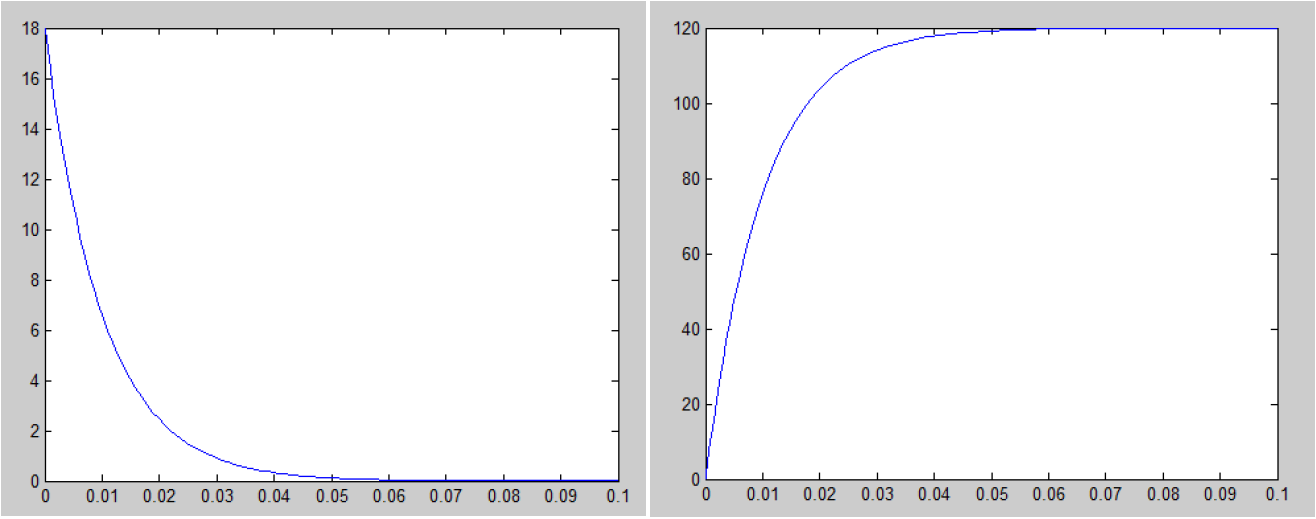
\includegraphics[scale=0.4]{TP2/TP2-Exo1a.PNG}
\end{center}

\Question
{
%question
\textit{Identifier l'élément du schéma (source E, capacité, résistance) auquel se rapportent ces deux graphes.}
}
{%correction
Attention, la réponse n'est valable que si l'on définit correctement la tension et le courant (module et sens):
\begin{center}
\begin{circuitikz} \draw
(0,0)	to[battery1, v=$E$, i^>=$i$, invert]	(0,3)
		to[closing switch, l=$t_0$] (3,3)
		to[C, l_=$C$, v^<=$V_C$]		(3,1.5)
		to[R, l=$R$]		(3,0)--(0,0)
;
\end{circuitikz}
\end{center}
La courbe de gauche représente le courant selon le sens choisi sur le schéma (en termes de forme, elle pourrait aussi représenter la ddp sur la résistance, mais dans ce cas la valeur de départ devrait être 120: il s'agit donc du courant) . La courbe de droite représente la ddp sur la capacité selon le sens choisi sur le schéma. Les valeurs initiales et finales sont importantes, ainsi que les asymptotes horizontales.
}


\Question
{
%question
\textit{Identifier la grandeur (tension(s), courant(s) ?) présente sur l'ordonnée de chaque graphe.}
}
{%correction
Sur la courbe de gauche, la valeur 18 représente un courant initial de 18A. En effet, le courant peut varier instantanément pour une capacité. Dans ce cas, il vaut simplement $\frac{120}{R}$, ce qui mène à $R=\frac{120}{18} \Omega$.\\
Sur la courbe de droite, 120 représente la tension de régime que va atteindre la capacité. En effet, suivant l'équation de maille $E=V_{C}+RI$, étant donné que le courant sera nul en régime (loi BF d'une capacité), la tension $V_{C}$ sera alors égale à $E$. 
}

Lors d'une autre mesure, la courbe suivante est relevée:
\begin{center}
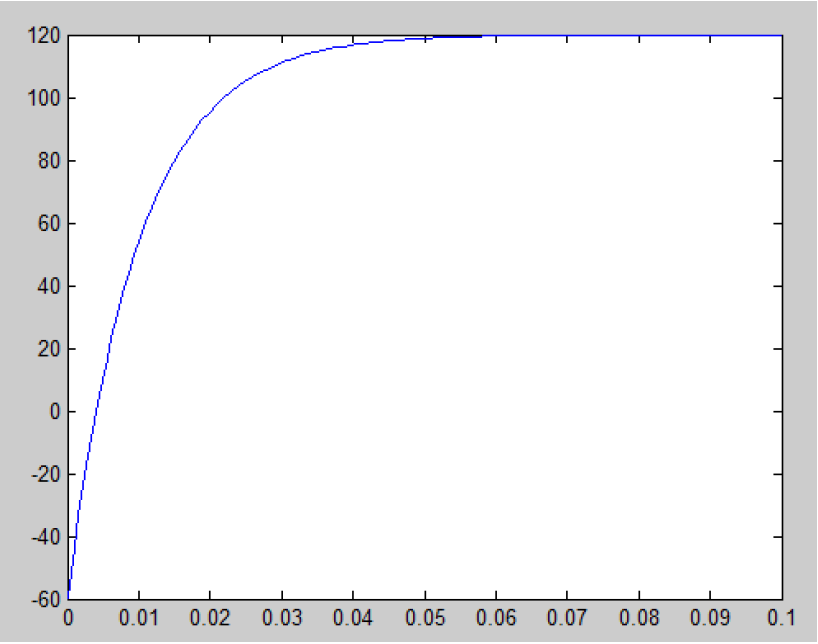
\includegraphics[scale=0.4]{TP2/TP2-Exo1b.PNG}
\end{center}

\Question
{
%question
\textit{Que représente-t-elle? Exliquer la présence de valeurs négatives et positives pour cette grandeur.}
}
{%correction
La courbe représente la tension aux bornes de la capacité. La charge initiale de celle-ci est telle que la tension est de -60V si on respecte le sens suivant pour la tension sur la capacité.
\begin{center}
\begin{circuitikz} \draw
(0,0)	to[battery1, v=$E$, i^>=$i$, invert]	(0,3)
		to[closing switch, l=$t_0$] (3,3)
		to[C, l_=$C$, v^<=$V_C$]		(3,1.5)
		to[R, l=$R$]		(3,0)--(0,0)
;
\end{circuitikz}
\end{center}
Il est intéressant de noter que la tension aux bornes de la capacité ne met pas plus de temps à atteindre sa valeur de régime lorsqu'elle a une charge initiale négative. En effet, ce temps est déterminé grâce à la constante de temps $\tau=RC$ qui est indépendante de la charge initiale.
}

\Question
{
%question
\textit{Si la capacité était remplacée par une inductance, quelle serait l'allure du courant du circuit et de la tension aux bornes de l'inductance?}
}
{%correction
L'allure de la tension aux bornes de l'inductance est d'allure semblable à celle du courant du circuit avec la capacité, et l'allure du courant dans le circuit avec l'inductance est semblable à celle de la tension aux bornes de la capacité.
}


\subsection{RC 2}
\Question
{
%question
\textit{Une capacité peut-elle fournir de l'énergie à un circuit?}
}
{%correction
Oui, elle peut restituer l'energie qu'elle a emmagasinée. Il s'agit de la tension initiale $V(0)$ qui agit alors comme une source qui fournit de l'énergie.
}

\begin{center}
\begin{circuitikz} \draw
(0,0)	to[battery1, v=$E$, invert]	(0,3)
		to[R, l_=$R$, v^<=$V_R$]		(3,3)
		to[C, l_=$C$, v^<=$V_C$]		(3,0)--(0,0)
;
\end{circuitikz}
\end{center}

\Question
{
%question
\textit{Pour le circuit suivant, est-il correct d'écrire:}\\
$$ V_{C}(t)=V(0)+\int_{0}^{t}\frac{1}{C}i(\xi)d\xi \hspace{1cm} ou \hspace{1cm} V_{C}(t)=V(0)-\int_{0}^{t}\frac{1}{C}i(\xi)d\xi \hspace{1cm} ?$$
}
{%correction
Pour répondre à cette question, il faut définir le sens du courant, sinon les deux expressions de $V_{C}$ ci-dessus n'ont aucun sens.
\begin{center}
\begin{circuitikz} \draw
(0,0)	to[battery1, v=$E$, i^>=$i$, invert]	(0,3)
		to[R, l_=$R$, v^<=$V_R$]		(3,3)
		to[C, l_=$C$, v^<=$V_C$]		(3,0)--(0,0)
;
\end{circuitikz}
\end{center}
Dans le cas ci-dessus, et en supposant $V(0)$ défini dans le même sens que $V_{C}$, la bonne expression est: 
$$V_{C}(t)=V(0)+\int_{0}^{t}\frac{1}{C}i(\xi)d\xi $$

Si le courant est défini dans le même sens que la tension par rapport à la capacité:
\begin{center}
\begin{circuitikz} \draw
(0,0)	to[battery1, v=$E$, i<=$i$, invert]	(0,3)
		to[R, l_=$R$, v^<=$V_R$]		(3,3)
		to[C, l_=$C$, v^<=$V_C$]		(3,0)--(0,0)
;
\end{circuitikz}
\end{center}
L'expression correcte est alors:\\
$$V_{C}(t)=V(0)-\int_{0}^{t}\frac{1}{C}i(\xi)d\xi $$
}


\subsection{RL}
%\ifthenelse{\boolean{assistant}}
%{\color{blue} Cet exercice n'est pas prioritaire.\\
%
%$\rightarrow$ Le but est de convaincre les étudiants que la loi $V=RI$ ne doit pas être utilisée pour tous les éléments. Il s’agit d’un raisonnement faux qui se base sur $V=RI$ appliqué  à une inductance. L’étudiant doit différencier la notion de modèle et d’élément réel (un fil a une certaine inductance et une bobine a une certaine résistance donc la discussion dépend du contexte). \\ \color{black}}{}


Pour le circuit suivant:
\begin{center}
\begin{circuitikz} \draw
(0,0)	to[battery1, v=$E$, invert]	(0,3)
		to[R, l_=$R$]		(3,3)
		to[L, l_=$L$]		(3,0)--(0,0)
;
\end{circuitikz}
\end{center}
\textit{Étant donné qu'une inductance est fondamentalement un fil bobiné d'une façon particulière, la loi d'Ohm peut lui être appliquée. Or, en régime permanent, comme la tension sur une inductance est nulle, on en conclut que, pour le circuit suivant, $i=0A$ en régime.}

\Question
{
%question
\textit{Expliquer pourquoi ce raisonnement (écrit en italique) est erroné.}
}
{%correction
Dans un schéma comme ci-dessus, R et L sont des dipôles idéaux. L'élément L est donc par définition une inductance pure répondant à la loi $V(t) = L \frac{di}{dt}$ et rien d'autre (il ne comprend en particulier pas de partie résistive). \\
Lorsque le texte évoque une inductance comme étant un fil bobiné, il évoque la version réelle d'une inductance, qu'on appellera plutôt une "bobine". Cette bobine possède à la fois un comportement inductif (comme une inductance pure) et un comportement résistif dû à la résistance du fil qui la constitue. Elle peut, dans sa globalité, être modélisée par l'ensemble R+L tel que dans le schéma ci-dessus. La bobine réelle est donc représentée ci-dessus par l'association d'une résistance pure et d'une inductance pure.\\
L'erreur du raisonnement est donc de confondre inductance réelle et inductance idéale: comme L dans le schéma représente une inductance idéale, la loi d'Ohm V=RI ne lui est pas applicable. Le fait que la tension soit nulle en régime sur L permet seulement de conclure que le courant sera constant en régime. (Il vaudra en particulier $E/R$)
}

\subsection{Du circuit aux équations}
%%assistant
%
%\ifthenelse{\boolean{assistant}}
%{\color{blue} Cet exercice n'est pas prioritaire.\\
%
%$\rightarrow$ Le but est de les habituer à différencier le comportement des inductances du comportement des capacités. Les conditions initiales pour la résolution d’équations différentielles semblent être un point sensible à l’examen. Le focus devrait donc être sur les conditions initiales.\\ \\ \color{black}}{}

Pour le circuit suivant:
\begin{center}
\begin{circuitikz} \draw
(0,0)	to[battery1, v=$E$, invert]			(0,4)
		to[closing switch, l=$t_0$] (2,4)
		to[C, l=$C$]				(2,2)
		to[R, l=$R_1$]				(2,0)
(2,4)--(4,4)
		to[L, l=$L$]				(4,2)
		to[R, l=$R_2$]				(4,0)--(0,0)
;
\end{circuitikz}
\end{center}

\Question
{
%question
\textit{Écrire les équations du circuit avant et après fermeture (fermeture en t=0) de l'interrupteur qui permettent de trouver les tensions et courants de tous les éléments.}
}
{%correction
Attention : ne pas oublier d'analyser ce qui se passe pour $t<0$, qui peut être très différent du comportement pour $t>0$. 

D'abord, on définit les courants et tensions en module et sens:
\begin{center}
\begin{circuitikz} \draw
(0,0)	to[battery1, v=$E$, i^>=$i_{tot}$, invert]			(0,4)
		to[closing switch, l=$t_0$] (2,4)
		to[C, l=$C$, v<=$V_C$, i=$i_1$]				(2,2)
		to[R, l=$R_1$, v<=$V_{R_1}$]				(2,0)
(2,4)--(4,4)
		to[L, l=$L$, i=$i_2$, v<=$V_L$]				(4,2)
		to[R, l=$R_2$, v<=$V_{R_2}$]				(4,0)--(0,0)
;
\end{circuitikz}
\end{center}
On peut alors faire le raisonnement suivant.

Avant la fermeture: l'interrupteur étant ouvert, la source de tension E est déconnectée des deux autres branches verticales du circuit et ne les influence pas. Dans l'absolu ceci ne veut pas dire qu'il ne peut pas y avoir de tension ou de courant dans ces branches. Cependant on peut observer que L et C sont en série (s'il y a un courant dans L c'est forcément le même dans C: $i_1 = -i_2$), or à long terme le courant est nul dans une capacité. Tous les courants sont donc nuls. En conséquence la ddp est nulle sur L et sur les deux R. Et comme ces trois éléments forment avec C une maille sur laquelle la tension totale doit être nulle, la ddp sur C est forcément nulle également. \\
Avant la fermeture, toutes les grandeurs électriques sont donc nulles dans les deux branches de droite. \\
N.B.: La ddp sur l'interrupteur vaut E pour vérifier la loi des mailles dans la maille de gauche.\\

Après fermeture :
$$E=V_{C}+V_{R_1}=V_{C}(0)+\int_{0}^{t}\frac{1}{C}i_1(\xi)d\xi+R_1i_{1}$$
$$E=V_{L}+V_{R_2}=L\frac{di_{2}}{dt}+R_2 i_{2}$$

Si l'on ne souhaite pas d'intégrale, on peut aussi écrire la première équation:
$$E=V_{C}+V_{R_1}=V_C+R_1 i_1=V_C + R_1 C\frac{dV_C}{dt}$$
}
\Question
{
%question
\textit{Donner les conditions initiales nécessaires à la résolution de ces équations.}
}
{%correction
Le courant dans l'inductance ne peut pas changer instantanément (loi HF d'une inductance):
$$i_{2}^{0+}=i_{2}^{0-}$$\\
et la tension aux bornes de la capacité ne peut pas changer instantanément (loi HF d'une capacité):
$$V_{C}^{0+}=V_{C}^{0-}$$\\
}

\subsection{Analyse qualitative}
%\ifthenelse{\boolean{assistant}}
%{\color{blue} Cet exercice n'est pas prioritaire.\\
%
%$\rightarrow$ Le but de cet exercice est d’étudier l’effet d’une résistance court-circuitée dans un circuit inductif. On s’attend à ce que l’étudiant pense qu’étant donné la présence d’une inductance dans le circuit, il est légitime de supposer que les courants i1 et i2 ne peuvent pas évoluer brutalement alors que c’est le courant total qui est soumis à la continuité du courant dans l’inductance.\\ \\ \color{black}}{}

Pour le circuit suivant:
\begin{center}
\begin{circuitikz} \draw
(0,0)	to[battery1, l=$E$, invert]			(0,6)
		to[closing switch, l=$t_0$, i=$i_1$]	(6,6)--(6,4)
		to[R, l=$R_2$]				(6,2)
		to[L, l=$L$]				(6,0)--(0,0)
(1,6)--(1,4)
		to[R, l=$R_1$, i=$i_2$]				(5,4)--(5,6)
;
\end{circuitikz}
\end{center}
Pour $t<0$, l'interrupteur est en position ouverte et le circuit est en régime. On ferme l'interrupteur à l'instant $t=t_0=0$, et on s'intéresse ensuite au temps $t>0$.

\Question
{
%question
\textit{Indiquer si les deux phrases suivantes sont correctes et justifier.
\begin{enumerate}
\item	La résistance totale du circuit (vue de la source) diminue après la fermeture de l'interrupteur.
\item	Étant donné qu'il y a une inductance dans le circuit:
	\begin{itemize}
	\item  le courant $i_{2}$ ne peut pas s'annuler directement lors de la fermeture du circuit: il passera (au signe près) progressivement de $\frac{E}{R_{1}+R_{2}}$ à $0A$.
	\item 	le courant $i_{1}$ passera immédiatement (au signe près) de $0 A$ à $\frac{E}{R_{2}}$ 	
	\end{itemize}
\end {enumerate}}
}
{%correction
\begin{enumerate}
\item	\textit{La résistance totale du circuit (vue de la source) diminue après la fermeture de l'interrupteur.}\\
%corrigé
La résistance totale du circuit passe de $R_{1}+R_{2}$ à $R_{2}$ étant donné qu'à partir de $t=0$, $R_{1}$ est court-circuitée. Le schéma équivalent de $R_1$ en parallèle avec l'interrupteur fermé est un court-circuit. Par conséquent, la résistance $R_{1}$ n'a plus aucun effet lors de l'étude du circuit, et l'affirmation est correcte.  
%fin corrigé
\item	\textit{Étant donné qu'il y a une inductance dans le circuit:}
\begin{itemize}
\item  \textit{le courant $i_{2}$ ne peut pas s'annuler directement lors de la fermeture du circuit: il passera (au signe près) progressivement de $\frac{E}{R_{1}+R_{2}}$ à $0A$.}\\
%corrigé
Le courant $i_{2}$ va s'annuler dès le moment où l'interrupteur est fermé ; il n'y a en effet aucune inductance dans cette partie du circuit. C'est en effet uniquement le courant qui parcourt l'inductance qui est régi par la loi de la continuité du courant.
\item 	\textit{le courant $i_{1}$ passera immédiatement (au signe près) de $0 A$ à $\frac{E}{R_{2}}$.}\\
%corrigé
Le courant $i_{1}$ va immédiatement passer de zéro à $\frac{E}{R1+R2}$ en $t=0$ étant donné que le courant dans une inductance est régi par

$$i_{inductance}^{0+}=i_{inductance}^{0-}$$

Il ne va donc pas prendre la valeur $\frac{E}{R_{2}}$ directement. Il s'agira de sa valeur de régime.
Le courant $i_{1}$ va donc passer directement de $0$ à $\frac{E}{R1+R2}$ étant donné qu'il s'agit du courant qui passe dans l'inductance avant fermeture et qu'il respecte la continuité du courant dans une inductance. Il va ensuite, à partir de cette valeur $\frac{E}{R1+R2}$, passer progressivement à sa valeur de régime $\frac{E}{R_{2}}$.
	\end{itemize}
\end {enumerate}
}

\subsection{Analyse et résolution d'un circuit}
%\ifthenelse{\boolean{assistant}}
%{\color{blue} Cet exercice n'est pas prioritaire.\\
%
%$\rightarrow$ Le but est de permettre aux étudiants de résoudre de A à Z un circuit réactif. Les trois premières questions font réaliser à l’étudiant que certains principes peuvent être utilisés afin de vérifier leurs résultats analytiques obtenus par la suite. Il est important de résoudre l’équation différentielle avec eux puisque cela requiert les conditions initiales. On s’attend également à ce que les étudiants appliquent les conditions initiales avant d’avoir trouvé la solution particulière.\\ \color{black}}{}

Pour t<0, le circuit suivant est en régime avec l'interrupteur ouvert. On ferme l'interrupteur en t=0.
\begin{center}
\begin{circuitikz} \draw
(0,0)	to[battery1, l=$E$, invert]			(0,2)
		to[R, l=$R_1$]				(2,2)
		to[closing switch, l=$t_0$]	(4,2)
		to[R, l=$R_2$]				(4,0)--(0,0)
(2,2)	to[C, l=$C$]				(2,0)
;
\end{circuitikz}
\end{center}

\Question
{
%question
\textit{Une capacité peut-elle se charger indéfiniment?}
}
{%correction
Non, que ce soit à cause de la topologie du circuit ou des limites physiques de la capacité.
}

\Question
{
%question
\textit{Que vaudra, en régime (avec l'interrupteur fermé), la tension aux bornes de la résistance $R_{2}$?}
}
{%correction
En régime, il n'y a pas de courant qui passe dans la capacité (loi BF). L'unique courant restant parcourra la maille comprenant la source de tension et les résistances $R_{1}$ et $R_{2}$ en série.\\
Nous avons donc $i=\frac{E}{R_{1}+R_{2}}$\\
La tension aux bornes de la résistance $R_{2}$ vaut $V_{R_{2}}=R_{2}i$\\
Ce qui nous donne  $V_{R_{2}}=E\frac{R_{2}}{R_{1}+R_{2}}$
}

\Question
{
%question
\textit{Est-il correct de dire que la condition initiale, en t=0, est exprimée par la tension nulle sur la résistance $R_{2}$ suivant le raisonnement suivant :\\
\og Le courant total de régime, au moment où l’interrupteur est fermé, est nul, puisqu’avant de fermer l’interrupteur, le circuit est en régime. Or, en régime, une capacité est analogue à un circuit ouvert. Comme $V=RI$ et qu'il n'y a pas de courant, la tension sur $R_{2}$ est bien nulle.\fg}
}
{%correction
C’est faux. La condition qu’impose la capacité est la continuité de la tension. La fermeture de l’interrupteur permet donc à un courant  de passer à travers la résistance $R_2$ étant donné qu’une différence de potentiel lui est appliquée. En régime, la tension sur la capacité avec l’interrupteur ouvert vaut E. Par conséquent, en t=0, une tension E sera également appliquée à la résistance $R_2$. 
$$V_{capa}^{0+}=V_{capa}^{0-}=R_{2}i_{R2}\hspace{5mm}(au\ signe\ pr\grave{e}s)$$
}

\Question
{
%question
\textit{Trouver les courants de branche du circuit pour tout instant.}
}
{%correction
\begin{center}
\begin{circuitikz} \draw
(0,0)	to[battery1, l=$E$, invert]		(0,2)
		to[R, l=$R_1$, i=$i$]								(2,2)
		to[closing switch, l=$t_0$]					(4,2)
		to[R, l=$R_2$, i=$i_2$]								(4,0)--(0,0)
(2,2)	to[C, l=$C$, i=$i_1$]								(2,0)
;
\end{circuitikz}
\end{center}

Avant fermeture de l'interrupteur: $R_2$ n'intervient pas car déconnectée du reste du circuit. Le courant dans $R_2$ est nul. En régime, le courant dans la capa est nul (loi BF), donc également dans $R_1$. La ddp sur $R_1$ est donc nulle également (loi d'Ohm). Et donc, par la loi des mailles, la ddp sur la capa vaut E.

Après fermeture de l'interrupteur:

Partons tout d'abord des équations de mailles :\\
$$E=R_{1}i+R_{2}i_{2}\hspace{1cm}(1)$$
$$V_{C}(0) + \frac{1}{C}\int_0^t i_1(\xi)d\xi =R_{2}i_{2}(t)\hspace{1cm}(2)$$
Et de l'équation des noeuds:
$$i=i_{1}+i_{2}\hspace{1cm}(3)$$
Grâce à $(1)$ et $(3)$ nous obtenons
$$E=R_{1}i_{1}+(R_{1}+R_{2})i_{2}$$
Et donc
$$i_{1}=\frac{E}{R_{1}}-\frac{R_{1}+R_{2}}{R_{1}}i_{2}$$
En dérivant $(2)$, nous obtenons
$$i_{1}(t)=CR_{2}\frac{di_{2}}{dt}$$

Ce qui mène à 
$$\frac{di_{2}}{dt}+\frac{R_{1}+R_{2}}{CR_{1}R_{2}}i_{2}=\frac{E}{CR_{1}R_{2}}$$


Nous allons commencer par calculer la solution générale de l'équation homogène (SGEH):
$$s+\frac{R_{1}+R_{2}}{CR_{1}R_{2}}=0$$
$$s=-\frac{R_{1}+R_{2}}{CR_{1}R_{2}}$$
$$i_{2_H}=A.e^{st}=A.e^{-\frac{R_{1}+R_{2}}{CR_{1}R_{2}}t}$$
\begin{center} où $A$ est une constante \end{center}

Nous allons ensuite calculer une solution particulière de l'équation non-homogène (SPEnH).
$$\frac{R_{1}+R_{2}}{CR_{1}R_{2}}i_{2_P}=\frac{E}{CR_{1}R_{2}}$$
$$i_{2_P}=\frac{E}{R_{1}+R_{2}}$$

La solution générale de l'équation non-homogène est la somme des SGEH et SPEnH 
$$i_2(t)=i_{2_H}(t)+i_{2_P}(t)=A.e^{-\frac{R_{1}+R_{2}}{CR_{1}R_{2}}t}+\frac{E}{R_{1}+R_{2}}$$
Il faut maintenant déterminer la valeur de la constante $A$. Nous savons que
$$i_{2}(t=0^{+})=\frac{V_{R_{2}}(t=0^{+})}{R_{2}}$$
Or nous savons que $V_{R_{2}}(t=0^{+})=V_{C}(t=0^{+})$.
Grâce à la loi HF de la capacité, nous avons
$$V_{C}(t=0^{+})=V_{C}(t=0^{-})$$
Comme nous sommes en régime en $t=0^{-}$, $V_{C}(t=0^{-})=E$. Nous avons donc
$$i_{2}(t=0^{+})=\frac{E}{R_{2}}$$
Ce qui nous donne
$$A=\frac{R_{1}}{R_{2}(R_{1}+R_{2})}E$$
La solution générale de l'équation non homogène est donc
$$i=\frac{R_{1}}{R_{2}(R_{1}+R_{2})}Ee^{-\frac{R_{1}+R_{2}}{CR_{1}R_{2}}t}+\frac{E}{R_{1}+R_{2}}$$
}

\Question
{
%question
\textit{Quels changements y a-t-il dans les conditions initiales si la capacité est remplacée par un inductance?}
}
{%correction
L'inductance imposera une continuité en courant. Elle est exprimée via:
$$i^{0+}_{inductance}=i^{0-}_{inductance}$$
}
\end{document}

% %% fancy header & foot
\pagestyle{fancy}
\lhead{[ELEC-H-2001] Électricité\\ TP \no 3 : Circuits linéaires et permanents avec source sinusoïdale\ifthenelse{\boolean{corrige}}{~-- corrigé}{}}
\rhead{v1.0.1\\ page \thepage}
\cfoot{}
%%

\pdfinfo{
/Author (Raoul Sommeillier, ULB -- BEAMS)
/Title (TP 3 ELEC-H-2001, Circuits linéaires et permanents soumis à une sollicitation sinusoïdale)
/ModDate (D:\pdfdate)
}

\hypersetup{
pdftitle={TP 3 [ELEC-H-2001] Électricité : Circuits linéaires et permanents soumis à une sollicitation sinusoïdale},
pdfauthor={Raoul Sommeillier, ©2018 ULB - BEAMS  },
%pdfsubject={filtrage et analyse fréquentielle}
}

%\date{\vspace{-1cm}\mydate\today}
%\title{\vspace{-2cm} Labo \no 6\\ Électronique appliquée [ELEC-H-301]\\Réalisation d'un ampli à transistor\ifthenelse{\boolean{corrige}}{~\\Corrigé}{}}

%\author{\vspace{-1cm}}%\textsc{Yannick Allard}}

\setlength{\parskip}{0.5cm plus4mm minus3mm} %espacement entre §
\setlength{\parindent}{0pt}


\begin{document}

\tptitle{}{Séance 3~: Circuits linéaires et permanents soumis à une sollicitation sinusoïdale}

\section{Pré-requis}
Avant la séance, vous aurez lu attentivement l'énoncé de la manipulation. Vous aurez par ailleurs relu les chapitres et sections suivants:

\begin{itemize}
	\item Chapitre 5 - Résoudre un circuit : procédure de base et accélérateur
	\begin{itemize}
		\item Section 5.1 - Vocabulaire lié aux circuits
		\begin{itemize}
			\item 5.1.2 Connexions série et parallèle 
			\item 5.1.3 Branche
			\item 5.1.4 Maille 
		\end{itemize}
		\item Section 5.2 - Lois de Kirchhoff
	\end{itemize}
	\item Chapitre 6 - Résoudre un circuit réactif dans le domaine temporel
	\begin{itemize}
		\item Section 6.5 - Analyse temporelle du circuit RL (source sinusoïdale)
		\item Section 6.6 - Analyse temporelle du circuit RLC
	\end{itemize}
	\item Chapitre 7 - Résoudre un circuit réactif dans le domaine fréquentiel
	\begin{itemize}
		\item Section 7.3 - Phaseur
		\item Section 7.4 - Impédances et admittances
		\begin{itemize}
			\item 7.4.2 Impédance d'une capacité pure
			\item 7.4.3 Impédance d'une résistance pure 
		\end{itemize}
	\end{itemize}

\end{itemize}

\vspace{5pt}

\newpage


\section{Exercices}
\subsection{RL}
La tension $e(t)=V_m \cos(\omega t+\alpha)$ est appliquée à l'instant $t=t_0=0$ au circuit $RL$.
\begin{center}
\begin{circuitikz} \draw
(0,0)	to[sinusoidal voltage source, v=$e(t)$, i^>=$i$]		(0,4)
		to[closing switch, l=$t_0$]		(3,4)
		to[R, l=$R$]					(3,2)
		to[L, l=$L$]					(3,0)--(0,0)
;
\end{circuitikz}
\end{center}

\Question
{%Q
\textit{Déterminer l'expression du courant $i(t)$ pour tout temps $t$ et discuter la valeur de $\alpha$ pour que:
\begin{enumerate}
\item le régime permanent s'établisse immédiatement
\item la valeur instantanée du courant soit maximale
\end{enumerate}}
}
{%C
La solution générale est (cfr cours):
$$i(t)=i'(t)+i''(t)=I_m \cos(\omega t + \alpha -\theta) - I_m \cos(\alpha -\theta) e^{-t/\tau}$$
Où $i'(t)$ est le terme de régime et $i''(t)$ le terme transitoire.

$$I_m=\frac{V_m}{\sqrt{{R^2}+(\omega L)^2}}$$
$$tan(\theta)=\frac{\omega L}{R}$$
$$\tau=\frac{L}{R}$$

Le transitoire est nul si $\cos(\alpha -\theta)=0 \Leftrightarrow \alpha -\theta=\pm \pi/2$.\\
Cela correspond à un enclenchement du circuit ($t=0$) au moment où le terme de régime passe par zéro. Dans ce cas, le régime permanent s'établit immédiatement.\\

Le terme transitoire sera maximum lorsque le circuit est enclenché au moment où le terme de régime passe par son maximum positif ou négatif ($\pm I_m$).
$$\alpha - \theta =0 \ ou \ \pi \Leftrightarrow i(t)=\pm I_m (\cos(\omega t) - e^{-\frac{R}{L}t})$$

Si $\omega L >> R$, le terme transitoire garde une valeur appréciable pendant plusieurs périodes.\\
Dans ce cas, le courant total atteint sa valeur maximale $i_{max}$ environ une demi-période après le branchement, lorsque le terme de régime s'approche de sa valeur maximale, mais a le même signe que le terme transitoire:
$$i_{max}=i(T/2)\simeq I_m (1+e^{-\frac{R}{L}\frac{T}{2}})=I_m (1+e^{-\pi \frac{R}{\omega L}}) \simeq 2I_m \ (si \frac{R}{\omega L}\ est\ petit)$$
\begin{center}
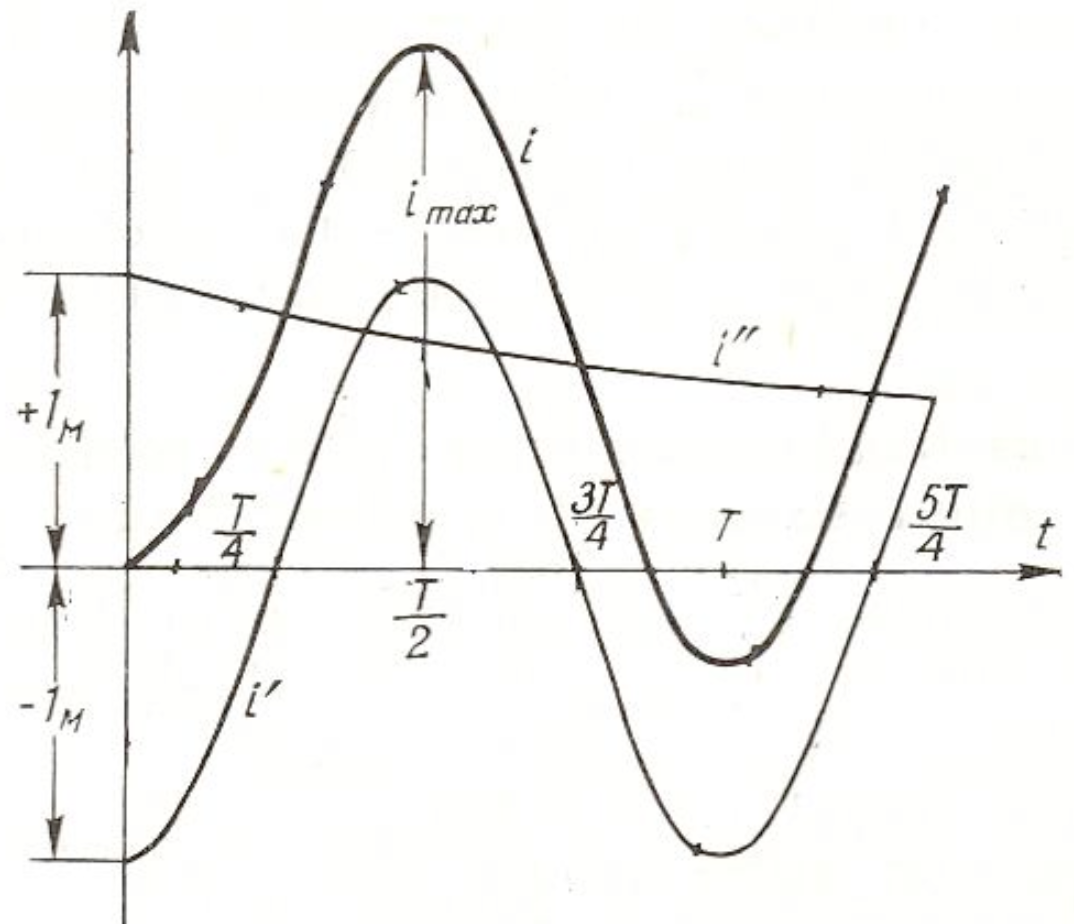
\includegraphics[scale=0.3]{TP3/TP3-Exo1.PNG}
\end{center}
}
{}


\subsection{Résoudre le circuit}
Pour le circuit suivant
\begin{center}
\begin{circuitikz} \draw
(0,0)	to[sinusoidal voltage source, v=$v_g(t)$]		(0,4)
		to[R, l=$R_1$]					(2,4)
		to[short]           (4,4)
(0,0)--(4,0)
		to[C, l=$C$, v>=$v_C(t)$]		(4,4)
(2,4)	to[R, l=$R_2$]					(2,2)
		to[L, l=$L$]					(2,0)
;
\end{circuitikz}
\end{center}
Où $v_g(t)=\sin (4t + 45^o)$, $R_1=4\Omega$, $R_2=1\Omega$, $L=1H$ et $C=\frac{1}{4}F$.

\Question
{%Q
\textit{Déterminer la tension aux bornes de la capacité en régime.}
}
{%C
\begin{center}
\begin{circuitikz} \draw
(0,0)	to[sinusoidal voltage source, v=$v_g(t)$, i^>=$i_g(t)$]		(0,4)
		to[R, l=$R_1$]					(2,4)
		to[short, i=$i_C(t)$]           (4,4)
(0,0)--(4,0)
		to[C, l=$C$, v>=$v_C(t)$]		(4,4)
(2,4)	to[R, l=$R_2$, i=$i_L(t)$]					(2,2)
		to[L, l=$L$]					(2,0)
;
\end{circuitikz}
\end{center}
Ayant défini les grandeurs dans le schéma, les lois des mailles, des noeuds et des composants permettent d'écrire:\\
$\underline{V}_g=R_1\underline{I}+\underline{V}_C=R_1(\underline{I}_L+\underline{I}_C)+\underline{V}_C$\\
$(R_2+j\omega L)\underline{I}_L=\underline{V}_C$\\
$\underline{V}_C=\frac{\underline{I}_C}{j\omega C}$

$\Rightarrow \underline{V}_C=\underline{V}_g \frac{R_2+j\omega L}{R_1(1-\omega^2LC)+R_2+j(\omega L+\omega CR_1R_2)}$

$\underline{V}_g=e^{j45^o}$ (avec des phaseurs en sinus comme dans l'énoncé, sinon déphaser de $90^o$)\\
$\Rightarrow \underline{V}_C=e^{j45^o}\frac{1+j4}{-11+j8}=e^{j45^o}\frac{4,12e^{j75,96^o}}{13,6e^{j143,97^o}}=0,303e^{-j23^o}$

L'expression finale en temporel est donc:\\ 
$v_C(t)=0,303 \sin(4t-23^o)$
}
{%A
}


\subsection{Résoudre le circuit 2}
Le circuit suivant se trouve en régime avant l'instant $t=t_0=0$ de fermeture de l'interrupteur. 
\begin{center}
\begin{circuitikz} \draw
(0,0)	to[sinusoidal voltage source, l=$e(t)$]		(0,2)
		to[R, l=$R_1$]								(2,2)
		to[closing switch, l=$t_0$]					(4,2)
		to[R, l=$R_2$]								(4,0)--(0,0)
(2,2)	to[C, l=$C$]								(2,0)
;
\end{circuitikz}
\end{center}
\Question
{%Q
\textit{Déterminer les courants pour toute valeur de $t$, avec $e(t)=E_0 \cos(\omega t)$.}
}
{%C
\begin{center}
\begin{circuitikz} \draw
(0,0)	to[sinusoidal voltage source, l=$e(t)$]		(0,2)
		to[R, l=$R_1$, i=$i_0$]								(2,2)
		to[closing switch, l=$t_0$]					(4,2)
		to[R, l=$R_2$, i=$i_2$]								(4,0)--(0,0)
(2,2)	to[C, l=$C$, i=$i_1$]								(2,0)
;
\end{circuitikz}
\end{center}

\begin{itemize}
\item \textbf{Pour $t<0$ (état de régime)}\\
$i_1(t)=i_0(t)$ et $i_2(t)=0$

$\underline{I}_0=\frac{E_0}{R_1+\frac{1}{j\omega C}}=\frac{j\omega CE_0}{1+j\omega CR_1}$\\
$\Rightarrow i_0(t)=\frac{\omega CE_0}{\sqrt{1+\omega^2 C^2 R_1^2}}\cos(\omega t+\phi)$ avec $tan(\phi)=\frac{1}{\omega CR_1}$\\

$\underline{V}_C=\frac{\underline{I}_0}{j\omega C}=\frac{E_0}{1+j\omega CR_1}$\\
$\Rightarrow v_C(t)=\frac{E_0}{\sqrt{1+\omega^2 C^2 R_1^2}}\cos(\omega t-\alpha)$ et $tan(\alpha)=\omega CR_1$
\item \textbf{Pour $t>0$}\\
$E_0 \cos(\omega t)=R_1(i_1+i_2)+R_2i_2$ \hspace{1cm}$(1)$\\
$v_C(0)+\frac{1}{C}\int_0^t i_1(\xi)d\xi=R_2i_2 \Rightarrow i_1=CR_2\frac{di_2}{dt}$\hspace{1cm}$(2)$\\
$(1)$ et $(2)$ $\Rightarrow E_0 \cos(\omega t)=(R_1+R_2)i_2+CR_1R_2\frac{di_2}{dt}$\\
$\Rightarrow i_2(t)=Ae^{-t\frac{R_1+R_2}{CR_1R_2}}+sol.\ partic.$\\

Pour chercher la solution particulière en $t>0$, $i_{2_p}(t)$, on va utiliser la méthode des phaseurs:\\
$\frac{1}{j\omega C}\underline{I}_1=R_2\underline{I}_2$\\
$\underline{E}_0=R_1(\underline{I}_1+\underline{I}_2)+R_2\underline{I}_2$\\

$\Rightarrow \underline{I}_2=\frac{E_0}{R_1+R_2+j\omega CR_1R_2}$\\
$\underline{I}_1=\frac{j\omega CR_2E_0}{R_1+R_2+j \omega CR_1R_2}$\\

La solution particulière est donc:\\
$$i_{2_p}(t)=K \cos(\omega t-\beta)$$
où $K=\frac{E_0}{\sqrt{(R_1+R_2)^2+(\omega CR_1R_2)^2}}$, $tan(\beta)=\omega \tau$ et $\tau=\frac{R_1R_2C}{R_1+R_2}$\\

La solution générale pour $t>0$ est alors:\\
$i_2(t)=Ae^{-t/\tau}+K \cos(\omega t-\beta)$\\
et il faut identifier $A$ à partir de la condition initiale.\\

\item \textbf{Condition initiale ($t=0^+$)}\\
$i_2(0^+)=\frac{v_C(0^+)}{R_2}=\frac{v_C(0^-)}{R_2}=\frac{E_0 \cos(\alpha)}{R_2\sqrt{1+\omega^2 C^2 R_1^2}}$\\
$A=\frac{E_0 \cos(\alpha)}{R_2\sqrt{1+\omega^2 C^2 R_1^2}}-K\cos(\beta)$\\

On a $i_2(t)$ pour $t>0$ (ouf!):\\
$i_2(t)=Ae^{-t/\tau}+K \cos(\omega t-\beta)$\\
$i_2(t)=\frac{E_0 \cos(\alpha)}{R_2\sqrt{1+\omega^2 C^2 R_1^2}}-K\cos(\beta)e^{-t\frac{R_1+R_2}{R_1R_2C}}+\frac{E_0}{\sqrt{(R_1+R_2)^2+(\omega CR_1R_2)^2}}\cos(\omega t-\beta)$

\item \textbf{Pour les autres courants en $t>0$}\\
$i_1(t)=CR_2\frac{di_2}{dt}=-\frac{CR_2}{\tau}Ae^{-t/\tau}-KCR_2\omega \sin(\omega t-\beta)$\\
$i_0(t)=i_1(t)+i_2(t)$
\end{itemize}
}
{%A
}


\subsection{Oscilloscope}
Le signal $V_e$ à mesurer est connecté à un oscilloscope au moyen d'une sonde externe. La sonde est constituée d'une résistance $R_S$ et d'une capacité $C_P$ (réglable) en parallèle.\\
L'impédance d'entrée de l'oscilloscope est modélisée par la mise en parallèle de $R_{in}=1M\Omega$ et $C_{in}=20pF$.\\
 
\begin{center}
\begin{circuitikz} \draw
node[ocirc] (A) at (0,2) {}
node[ocirc] (B) at (0,0) {}
(B) to [open, v^=$V_e$] (A)
node[ocirc] (C) at (3.5,2) {}
node[ocirc] (D) at (3.5,0) {}
(D) to [open, v^=$V_{in}$] (C)
(0,2)--(1,2)
		to[R, l=$R_S$]		(3,2)--(7,2)
		to[C, l=$C_{in}$]	(7,0)
(5,2)	to[R, l=$R_{in}$]	(5,0)
(1,2)--(1,3.5)
		to[variable capacitor, l=$C_P$, mirror]	(3,3.5)--(3,2)
(0,0)--(5,0)	
(5,0) node[ground] {}
(7,0) node[ground] {}
node[]() at (6.25,4){Oscilloscope}
;
\draw[dashed](4,-1)--(4,5)--(8.5,5)--(8.5,-1)--(4,-1);
\end{circuitikz}
\end{center}
\Question
{%Q
\textit{Déterminer les éléments de la sonde pour réaliser un facteur de division de $k$ (par exemple $k=10$) sans déformer le signal mesuré.\\
Dans ces conditions, déterminer la nouvelle impédance d'entrée équivalente.}
}
{%C
La sonde (externe) à haute impédance permet de connecter le signal à étudier à l'oscilloscope tout en réalisant un facteur de division (par exemple 10 ou 100) indépendant de la fréquence.\\
La sonde est constituée d'une résistance $R_S$ fixe et d'un condensateur $C_P$ réglable.\\

Le rapport de division est:\\
$$\frac{\underline{V}_{in}}{\underline{V}_e}=\frac{Z_{in}}{Z_S+Z_{in}}=\frac{1}{1+\frac{R_S}{R_{in}}\frac{1+j\omega R_{in}C_{in}}{1+j\omega R_{S}C_{P}}}$$

Pour que le signal à l'entrée de l'oscilloscope ne soit pas déformé, il faut que ce rapport soit indépendant de la fréquence (la sonde sera alors dite \underline{adaptée}):\\
$$R_SC_P=R_{in}C_{in} \hspace{1cm} (1)$$

Le rapport $\frac{1}{k}=\frac{\underline{V}_{in}}{\underline{V}_e}=\frac{R_{in}}{R_S+R_{in}}$ sera réel et indépendant de $\omega$. On aura donc:\\
$$R_S=(k-1)R_{in} \ et \ C_P=\frac{C_{in}}{k-1}$$
où $k$ est le \underline{rapport d'atténuation} de la sonde.\\

Exemple: $R_{in}=1M\Omega$, $C_{in}=20pF$, $k=10$ $\Rightarrow R_S=9M\Omega$ et $C_P=2,2pF$\\

Si la condition d'adaptation $(1)$ de la sonde est réalisée, l'impédance d'entrée de l'oscilloscope muni de la sonde est:\\
$$Z_e=Z_{in}+Z_S=\frac{R_{in}}{1+j\omega R_{in}C_{in}}+\frac{R_{S}}{1+j\omega R_{S}C_{P}}=\frac{R_{in}+R_S}{1+j\omega (R_{in}+R_S) \frac{C_{in}C_P}{C_{in}+C_P}}$$

La résistance d'entrée et la capacité d'entrée sont devenues:\\
$$R_e=R_{in}+R_S=kR_{in}$$
$$C_e=\frac{C_{in}C_P}{C_{in}+C_P}=\frac{C_{in}}{k}$$\\

La sonde permet donc d'augmenter la résistance d'entrée et de diminuer la capacité d'entrée.\\

Pour l'exemple: $R_e=10M\Omega$ et $C_e=2pF$.
}
{}

\subsection{RLC}
Pour le circuit RLC série en régime sinusoïdal permanent suivant:
\begin{center}
\begin{circuitikz} \draw
(0,0)	to[sinusoidal voltage source, v=$V_g$]		(0,3)
		to[R, l=$R$, v<=$V_R$]		(3,3)
		to[L, l=$L$, v<=$V_L$]		(6,3)
		to[C, l=$C$, v<=$V_C$]		(6,0)--(0,0)
;
\end{circuitikz}
\end{center}
\Question
{%Q
\textit{Représenter les phaseurs des différentes tensions dans le plan complexe (diagramme des phaseurs), en prenant le courant comme origine des phases. On se placera successivement dans le cas $\omega > \omega_0$, $\omega < \omega_0$, $\omega = \omega_0$, avec $\omega = \frac{1}{LC}$.}
}
{%C
$\underline{V}_g=\underline{V}_R+\underline{V}_L+\underline{V}_C$\\
$\underline{V}_R=R\underline{I}$\\
$\underline{V}_L=j\omega L\underline{I}$\\
$\underline{V}_C=-j\frac{1}{\omega C}\underline{I}$
$$\Rightarrow \underline{I}=\frac{\underline{V}_g}{Z}=\frac{\underline{V}_g}{R+j(\omega L-\frac{1}{\omega C})}$$

\begin{itemize}
\item $\omega>\omega_0 \Rightarrow |\underline{V}_L|>|\underline{V}_C|$\\
Le circuit est globalement inductif et le courant est en retard (de $\theta$) sur la tension.
\item $\omega<\omega_0 \Rightarrow |\underline{V}_L|<|\underline{V}_C|$\\
Le circuit est globalement capacitif et le courant est en avance sur la tension.
\item $\omega=\omega_0 \Rightarrow |\underline{V}_L|=|\underline{V}_C|$\\
Les réactances inductive et capacitive se compensent exactement. Le courant et la tension sont en phase.
\end{itemize}
\begin{center}
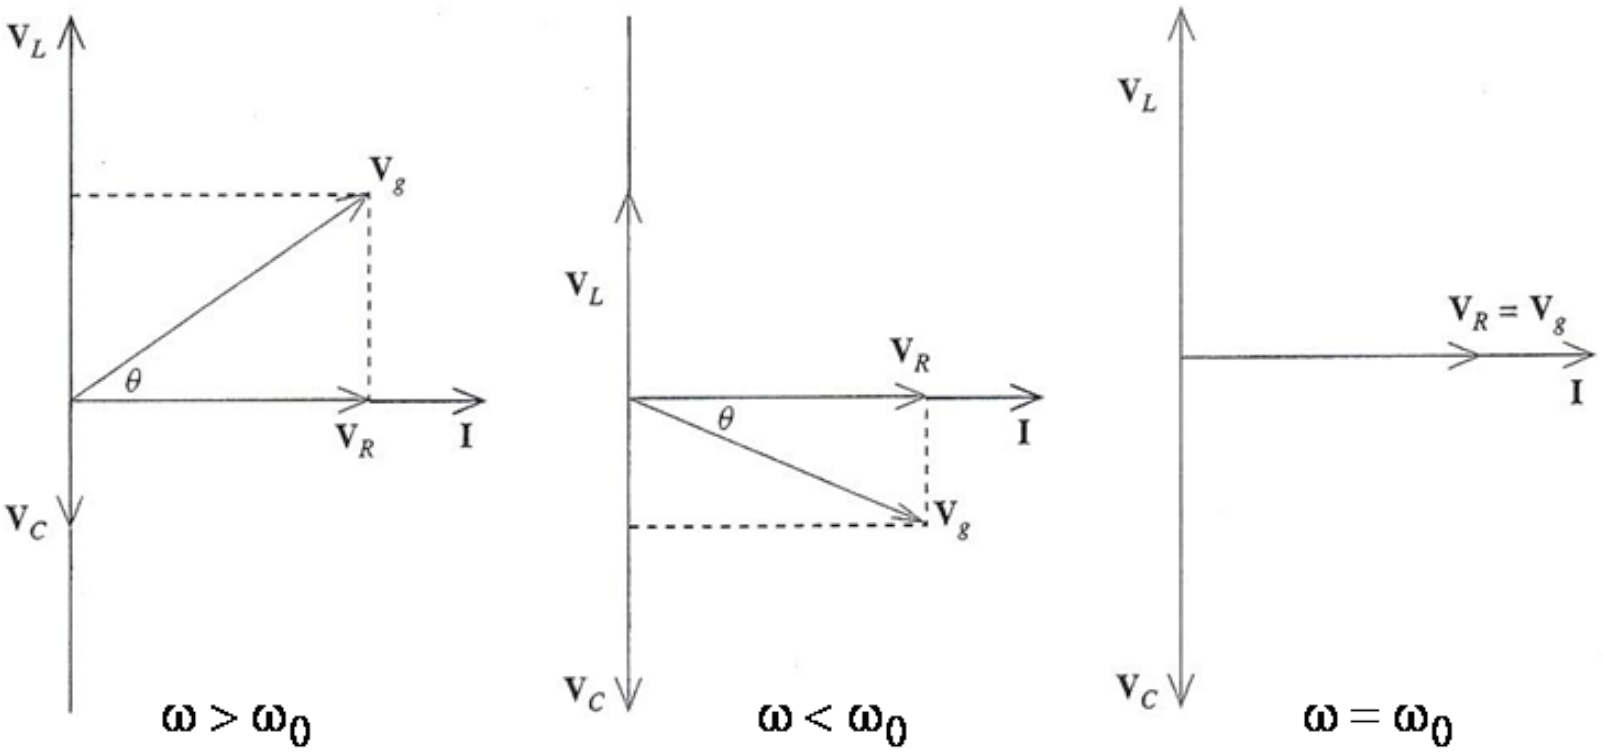
\includegraphics[scale=0.3]{TP3/TP3-Exo5.PNG}
\end{center}
}{}

\Question
{%Q
\textit{La tension $V_C$ peut-elle devenir supérieure à la tension d'alimentation?}
}
{%C
Affirmatif, c'est le principe de la résonance.\\
$V_C$ (et $V_L$) peuvent devenir supérieures à $V_g$. Par contre, $V_R$ ne peut pas dépasser $V_g$.
}



\end{document}
% %% fancy header & foot
\pagestyle{fancy}
\lhead{[ELEC-H-2001] Électricité\\ TP \no 4 : Théorèmes de superposition et de Thévenin, et Mutuelles\ifthenelse{\boolean{corrige}}{~-- corrigé}{}}
\rhead{v1.0.2\\ page \thepage}
\cfoot{}
%%

\pdfinfo{
/Author (Raoul Sommeillier, ULB -- BEAMS)
/Title (TP 4 ELEC-H-2001, Théorème de superposition, théorème de Thévenin et Mutuelles)
/ModDate (D:\pdfdate)
}

\hypersetup{
pdftitle={TP 4 [ELEC-H-2001] Électricité : Théorème de superposition, théorème de Thévenin et Mutuelles},
pdfauthor={Raoul Sommeillier, ©2018 ULB - BEAMS  },
%pdfsubject={filtrage et analyse fréquentielle}
}

%\date{\vspace{-1cm}\mydate\today}
%\title{\vspace{-2cm} Labo \no 6\\ Électronique appliquée [ELEC-H-301]\\Réalisation d'un ampli à transistor\ifthenelse{\boolean{corrige}}{~\\Corrigé}{}}

%\author{\vspace{-1cm}}%\textsc{Yannick Allard}}

\setlength{\parskip}{0.5cm plus4mm minus3mm} %espacement entre §
\setlength{\parindent}{0pt}


\begin{document}

\tptitle{}{Séance 4~: Théorème de superposition, théorème de Thévenin et Mutuelles}

\section{Pré-requis}
Avant la séance, vous aurez lu attentivement l'énoncé de la manipulation. Vous aurez par ailleurs relu les chapitres et sections suivants:
\begin{itemize}
	\item Chapitre 3 - Quadripôles idéaux
		\begin{itemize}
		\item Section 3.3 - Inductance mutuelle et transformateur idéal
		\end{itemize}
	\item Chapitre 4 - Équivalence de Thévenin et adaptation d’impédance
		\begin{itemize}
		\item Section 4.1 - Circuits équivalents et théorèmes de Thévenin/Norton
			\begin{itemize}
			\item 4.1.2 Théorème et équivalent de Thévenin (Exemple : Retour sur le diviseur résistif)
			\end{itemize}
		\end{itemize}
	\item Chapitre 5 - Résoudre un circuit : procédure de base et accélérateurs
		\begin{itemize}
		\item Section 5.1 - Vocabulaire lié aux circuits
			\begin{itemize}
			\item 5.1.4 Maille
			\end{itemize}
		\item Section 5.2 - Lois de Kirchhoff
		\item Section 5.8 - Théorème de superposition
		\end{itemize}
	\item Chapitre 7 - Résoudre un circuit réactif dans le domaine fréquentiel
		\begin{itemize}
		\item Section 7.3 - Phaseurs
		\end{itemize}
\end{itemize}

\vspace{5pt}

\newpage

\section{Exercices}
\subsection{Exercice 1}

Le circuit suivant est alimenté par la f.e.m. $e(t)= E_{0}+E_{1}sin(\omega t)+E_{2}sin(2\omega t+\phi)$.
\begin{center}
\begin{circuitikz} \draw
(0,0)   to[sV, v=$e(t)$] 	(0,3)--(6,3)
		to[C, l=$C$] (6,1.5)
		to[R, l=$R_C$] (6,0)--(0,0)
(3,3)   to[L, l=$L$] (3,1.5)
		to[R, l=$R_L$](3,0)
;
\end{circuitikz}
\end{center}

\Question
{%Question
\textit{Déterminer les expressions temporelles des courants de chaque branche du circuit.}
}
{%CorrigŽ
Étant donné qu'il s'agit d'une f.e.m. composée de signaux à différentes fréquences, nous allons appliquer le théorème de superposition. 

\begin{enumerate}

\item $e(t)=E_{0}$ ($\omega=0\ rad/s$) \\
Étant donné qu'il s'agit d'une source de tension continue et que nous sommes en régime, une capacité peut être assimilée à un circuit ouvert et une inductance peut être assimilée à un court circuit. Nous avons donc:
$I_{C_{0}}=0$ et $I_{L_{0}}=I_{R_L}=\frac{E_{0}}{R_L}$

\item $e(t)=E_{1}sin(\omega t)$ (pulsation: $\omega_1=\omega\ rad/s$)\\
Il ne s'agit plus d'une source continue et nous sommes en régime. Nous allons donc utiliser les phaseurs.
$$\underline{I_1}=\underline{I}_{L_{1}}+\underline{I}_{C_{1}}$$
$$\underline{E}_{1}=(R_{L}+j\omega_{1} L)\underline{I}_{L_{1}}$$
$$\underline{E}_{1}=(R_{C}+\frac{1}{j\omega_{1} C})\underline{I}_{C_{1}}$$ 

$$\Leftrightarrow \underline{I}_{L_{1}}=\frac{\underline{E}_{1}}{R_{L}+j\omega_{1} L}$$
$$\hspace{9mm} \underline{I}_{C_{1}}=\frac{j\omega_{1} C\underline{E}_{1}}{1+j\omega_{1} CR_{C}}$$

$$\Leftrightarrow I_{{L}_1}=|\underline{I}_{L_{1}}|=\frac{E_{1}}{\sqrt{R_{L}^{2}+(\omega_1 L)^{2}}}=\frac{E_{1}}{\sqrt{R_{L}^{2}+(\omega L)^{2}}}$$
$$I_{{C}_1}=|\underline{I}_{C_{1}}|=\frac{\omega_1 CE_{1}}{\sqrt{1+(\omega_1 CR_{C})^{2}}}=\frac{\omega CE_{1}}{\sqrt{1+(\omega CR_{C})^{2}}}$$

$$\Leftrightarrow \phi_{I_{L_{1}}}= Arg(\underline{I}_{L_{1}})=Arg(\underline{E}_1)-Arg(R_{L}+j\omega_{1} L)=0-arctg(\frac{\omega_{1} L}{R_{L}})=-arctg(\frac{\omega L}{R_{L}})$$
$$\phi_{I_{C_{1}}}= Arg(\underline{I}_{C_{1}})=Arg(j\omega_{1} C)+Arg(\underline{E}_1)-Arg(1+j\omega_{1} CR_{C})=\frac{\pi}{2}+0-arctg(\omega_{1} CR_C)=\frac{\pi}{2}-arctg(\omega CR_C)$$

\item $e(t)=E_{2}sin(2\omega t+\phi)$ (pulsation: $\omega_{2}=2\omega\ rad/s$)\\
La source se situant au même endroit que précédemment, inutile de refaire tous les calculs. Il suffit de modifier la pulsation et de tenir compte de la phase $\phi$ de la source de tension.\\

$$\underline{I}_{L_{2}}=\frac{\underline{E}_{2}}{R_{L}+j\omega_{2} L}$$
$$\underline{I}_{C_{2}}=\frac{j\omega_{2} C\underline{E}_{2}}{1+j\omega_{2} CR_{C}}$$
$$\underline{I}_2=\underline{I}_{L_{2}}+\underline{I}_{C_{2}}$$

$$\Leftrightarrow I_{{L}_2}=|\underline{I}_{L_{2}}|=\frac{E_{2}}{\sqrt{R_{L}^{2}+(\omega_2 L)^{2}}}=\frac{E_{2}}{\sqrt{R_{L}^{2}+(2\omega L)^{2}}}$$
$$I_{{C}_2}=|\underline{I}_{C_{2}}|=\frac{\omega_2 CE_{2}}{\sqrt{1+(\omega_2 CR_{C})^{2}}}=\frac{2\omega CE_{2}}{\sqrt{1+(2\omega CR_{C})^{2}}}$$

$$\Leftrightarrow \phi_{I_{L_{2}}}= Arg(\underline{I}_{L_{2}})=Arg(\underline{E}_2)-Arg(R_{L}+j\omega_{2} L)=\phi-arctg(\frac{\omega_{2} L}{R_{L}})=\phi-arctg(\frac{2\omega L}{R_{L}})$$
$$\phi_{I_{C_{2}}}= Arg(\underline{I}_{C_{2}})=Arg(j\omega_{2} C)+Arg(\underline{E}_2)-Arg(1+j\omega_{2} CR_{C})=\frac{\pi}{2}+\phi-arctg(2\omega CR_C)$$

\item Superposition:\\\\
$$\Rightarrow i_{L}(t)=I_{L_{0}}+ i_{L_{1}}(t)+i_{L_{2}}(t)=\frac{E_{0}}{R_{L}}+I_{{L}_1}sin(\omega t+\phi_{I_{L_{1}}})+I_{{L}_2}sin(2\omega t+\phi_{I_{L_{2}}})$$
$$=\frac{E_{0}}{R_{L}}+\frac{E_{1}}{\sqrt{R_{L}^{2}+(\omega L)^{2}}}sin(\omega t-arctg(\frac{\omega L}{R_{L}}))+\frac{E_{2}}{\sqrt{R_{L}^{2}+(2\omega L)^{2}}}sin(2\omega t+\phi-arctg(\frac{2\omega L}{R_{L}}))$$

$$\Rightarrow i_{C}(t)=I_{C_{0}}+ i_{C_{1}}(t)+i_{C_{2}}(t)=I_{{C}_1}sin(\omega t+\phi_{I_{C_{1}}})+I_{{C}_2}sin(2\omega t+\phi_{I_{C_{2}}})$$
$$=\frac{\omega CE_{1}}{\sqrt{1+(\omega CR_{C})^{2}}}sin(\omega t+\frac{\pi}{2}-arctg(\omega CR_C))+\frac{2\omega CE_{2}}{\sqrt{1+(2\omega CR_{C})^{2}}}sin(2\omega t+\frac{\pi}{2}+\phi-arctg(2\omega CR_C))$$

$$\Rightarrow i(t)=i_{C}(t)+i_{L}(t)$$
\end{enumerate}
}
%

\subsection{Exercice 2}

Soit le circuit suivant, comportant une source de tension $e(t)=2sin(5000t)$ et une source de courant $i_{S}(t)=cos(10000t)$:
\begin{center}
\begin{circuitikz} \draw
(0,0)   to[american voltage source, v>=$e(t)$, invert] 	(0,3)
		to[R, l=$R_1$] (2,3)
		to[C, l=$C$] (4,3)--(8,3)

		to[american current source, l_=$i_S$] (8,0)--(0,0)
(4,0)	to[battery1, v>=$3V$, invert] (4,1.5)
		to[R, l=$R_2$] (4,3)
(6,0)	to[L, l=$L$] (6,1.5)
		to[R, l=$R_3$] (6,3)
node[ocirc] (A) at (8.5,3) {}
node[ocirc] (B) at (8.5,0) {}
(B) to [open, v_=$v(t)$] (A)	
;
\end{circuitikz}
\end{center}
Où $R_1=4\Omega$, $R_2=2 \Omega$, $R_3=4\Omega$, $C=10\mu F$ et $L=1mH$.

\Question
{%question
\textit{Déterminer l'expression temporelle de la tension $v(t)$ de ce circuit.}
}
{%corrigŽ
Étant donné qu'il s'agit de différentes sources à différentes fréquences, nous allons appliquer le théorème de superposition.

\begin{itemize}

\item Source continue seule ($\omega = \omega_0 = 0rad/s$): on annule les autres sources \\

Étant donné qu'il s'agit d'une source de tension continue et que nous sommes en régime, une capacité peut être assimilée à un circuit ouvert et une inductance peut être assimilée à un court circuit. Nous avons donc le schéma suivant:
\begin{center}
\begin{circuitikz} \draw
(0,0)   to[short, l=$e(t)$] 	(0,3)
		to[R, l=$R_1$] (2,3)
		to[open, l=$C$] (4,3)--(8,3)

		to[open, l_=$i_S$] (8,0)--(0,0)
(4,0)	to[battery1, v>=$3V$, invert] (4,1.5)
		to[R, l=$R_2$] (4,3)
(6,0)	to[short, l=$L$] (6,1.5)
		to[R, l=$R_3$] (6,3)
node[ocirc] (A) at (8.5,3) {}
node[ocirc] (B) at (8.5,0) {}
(B) to [open, v_=$v(t)$] (A)	
;
\end{circuitikz}
\end{center}
\vspace{3mm}
Il s'agit alors d'une simple maille avec deux résistances. $v(t)$ est la tension aux bornes de $R_{3}$. Nous avons un diviseur résistif et donc:
$$v_0(t)=\frac{R_{3}}{R_{2}+R_{3}}10V=2V$$

\item Source de tension $e(t)$ seule ($\omega = \omega_1 = 5000rad/s$) 
\begin{center}
\begin{circuitikz} \draw
(0,0)   to[american voltage source, v>=$e(t)$, invert] 	(0,3)
		to[R, l=$R_1$] (2,3)
		to[C, l=$C$] (4,3)--(8,3)

		to[open, l_=$i_S$] (8,0)--(0,0)
(5,0)	to[generic, l=$Z$] (5,3)

node[ocirc] (A) at (8.5,3) {}
node[ocirc] (B) at (8.5,0) {}
(B) to [open, v_=$v(t)$] (A)	
;
\end{circuitikz}
\end{center}

\end{itemize}

Afin de réduire le circuit à une maille, $Z$ est la mise en parallèle de ($R_{3}$ et $L$, en série) avec $R_{2}$.
$$Z=R_2//(R_3+L)=\frac{R_{2}(R_{3}+j\omega_1 L)}{R_{2}+R_{3}+j\omega_1 L}=1,64.e^{j.11,5^{o}} [\Omega]$$
	$$\underline{V}=\underline{E}\frac{Z}{R_{1}+\frac{1}{j\omega_1 C}+Z}=0,16.e^{j.85,6^{o}}$$
	Nous avons donc:
	$$v_1(t)=0,16.sin(5000t+85,6^{o}) [V]$$
	\begin{itemize}
	\item Source de courant $i_{S}(t)$ seule. \\
	Soit $Z'$ l'impédance vue par la source $i_{S}(t)$.
	\begin{center}
	\begin{circuitikz} \draw
	(0,0)   to[generic, l=$Z'$] 	(0,2)--(2,2)
			to[american current source, l_=$i_S$] (2,0)--(0,0)

	node[ocirc] (A) at (2.5,2) {}
	node[ocirc] (B) at (2.5,0) {}
	(B) to [open, v_=$v(t)$] (A)	
	;
	\end{circuitikz}
	\end{center}
	$$Z'=(R_1+C)//R_2//(R_3+L)=\frac{1}{\frac{1}{R_{1}+\frac{1}{j\omega_{2}C}}+\frac{1}{R_{2}}+\frac{1}{R_{3}+j\omega_{2}L}}=1,758 [\Omega]$$
	Compte tenu des sens déjà définis pour v(t) et de $i_S$, ces deux grandeurs correspondent sur Z' à une convention \underline{générateur}. Il faut donc pour Z'utiliser un signe négatif dans la loi d'Ohm généralisée :
	$$\underline{V}=-Z'\underline{I_{S}}=-1,758$$
	$$v_2(t)=-1,758cos(1000t) [V]$$
	Par superposition, la solution totale est donc:\\
	$$v(t)= v_0(t)+v_1(t)+v_2(t)=2+0,16sin(5000t+85,6^{o})-1,758cos(1000t) [V]$$
	\end{itemize}
}
%

\subsection{Exercice 3}
Soit le circuit suivant:
\begin{center}
\begin{circuitikz} \draw
(0,0)   to[sV, v>=$e(t)$] 	(0,3)
		to[R, l=$R$] (2,3)--(6,3)
		to[generic, l=$Z$, i=$i(t)$] (6,0)--(0,0)
(2,3)	to[C, l=$C$] (2,0)
(4,3)	to[R, l=$R$] (4,0)
;
\end{circuitikz}
\end{center}

\Question
{%Question
\textit{Déterminer le courant $i(t)$ dans le circuit suivant en appliquant le théorème de Thévenin}.
}
{%Cor
Équivalent de Thévenin du circuit à gauche de $Z$:
$$Z_{th}=\frac{1}{\frac{1}{R}+\frac{1}{R}+j\omega C}=\frac{R}{2+j\omega CR}$$\\
La tension $E_{Th}$ est la tension aux bornes de la résistance $R$ verticale (égale à la tension sur $C$, puisque en parallèle). Nous avons donc:
$$\underline{E}_{Th}=\frac{\frac{R}{1+j\omega CR}\underline{E}}{R+\frac{R}{1+j\omega CR}}=\frac{\underline{E}}{2+j\omega CR}$$
Pour trouver la valeur du courant dans le circuit, nous relions l'équivalent de Thévenin avec l'impédance $Z$. Nous avons donc:
$$\underline{I}=\frac{\underline{E}_{Th}}{Z_{Th}+Z}=\frac{\underline{E}}{R+Z(2+j\omega CR)}$$
}
{%Assist
}

\Question
{%Q
\textit{Si l'impédance $Z$ est telle que $Z=R+jX$, quelle condition doit satisfaire cette impédance pour que le courant $i(t)$ ne soit pas déphasé par rapport à la source $e(t)=Ecos(\omega t)$?}
}
{%C
Puisque $Z=R+jX$, nous avons:
$$\underline{I}=\frac{\underline{E}}{(R+2R-\omega CRX)+j(\omega CR^2+2X)}$$
Un déphasage nul entre le courant et la tension correspond à une partie imaginaire nulle dans l'expression du phaseur $\underline{I}$ ci-dessus. La condition est donc que:
$$X=-\frac{1}{2}\omega CR^2$$
}
{%A
}

\subsection{Exercice 4}
Soit un circuit inconnu dont deux bornes sont accessibles. Lors d'une première expérience, les deux bornes sont laissées ouvertes et on mesure une tension de phaseur $\underline{V_{1}}$. Lors d'une deuxième expérience, une résistance $R_{u}$ est connectée et le phaseur associé à la tension mesurée vaut $\underline{V_{2}}$. 
\begin{center}
\begin{circuitikz} \draw
(2,1.75)--(3,1.75)
(2,0.25)--(3,0.25)
(0,0)--(0,2)--(2,2)--(2,0)--(0,0)
node[ocirc] (A) at (3,1.75) {}
node[ocirc] (B) at (3,0.25) {}
(B) to [open, v_=$v_1(t)$] (A)
;
\end{circuitikz}
\hspace{1cm}
\begin{circuitikz} \draw
(2,1.75)--(3,1.75)--(4.75,1.75) to[R, l=$R_u$] (4.75,0.25)--(3,0.25)
(2,0.25)--(3,0.25)
(0,0)--(0,2)--(2,2)--(2,0)--(0,0)
node[ocirc] (A) at (3,1.75) {}
node[ocirc] (B) at (3,0.25) {}
(B) to [open, v_=$v_2(t)$] (A)
;
\end{circuitikz}
\end{center}


\Question
{%Q
\textit{Déterminer l'équivalent de Thévenin du circuit vu au travers des deux bornes.}
}
{%C
\begin{center}
\begin{circuitikz} \draw
(0,0)	to[sinusoidal voltage source, v=$\underline{E}_{th}$] (0,2)
		to[generic, l=$Z$] (3,2)
(0,0)--(3,0)

node[ocirc] (A) at (3,2) {}
node[ocirc] (B) at (3,0) {}
(B) to [open, v_=$v_1(t)$] (A)
;
\end{circuitikz}
\hspace{1cm}
\begin{circuitikz} \draw
(0,0)	to[sinusoidal voltage source, v=$\underline{E}_{th}$] (0,2)
		to[generic, l=$Z$] (3,2)
(0,0)--(3,0)
node[ocirc] (A) at (3,2) {}
node[ocirc] (B) at (3,0) {}
(B) to [open, v_=$v_2(t)$] (A)
(3,2)--(4.75,2) to[R, l=$R_u$] (4.75,0)--(3,0)
;
\end{circuitikz}
\end{center}
\begin{itemize}
\item Pour la première expérience, nous avons un circuit ouvert. Nous avons donc:
$$\underline{V}_{1}=\underline{E}_{Th}$$
\item Pour la seconde expérience, $\underline{V}_{2}$ est la tension aux bornes de la résistance $R_{u}$. Nous avons donc:
$$\underline{V}_{2}=\frac{R_{u}}{R_{u}+Z_{Th}}\underline{E}_{Th}$$ et 
$$Z_{Th}=R_u(\frac{\underline{E}_{Th}}{\underline{V}_{2}}-1)$$
\end{itemize}
}
{%A
}

\subsection{Exercice 5}
Soit le circuit suivant:
\begin{center}
\begin{circuitikz} \draw
(0,0)	to[sinusoidal voltage source, v=$e(t)$] (0,3)
		to[R, l=$R_1$] (2,3)
		to[L, l=$L_1$] (4,3)
		to[L, l=$L_2$] (4,1.5)
		to[C, l=$C$] (4,0)--(0,0)
node[circ] (A) at (3.75,1.5) {}
node[circ] (B) at (2.25,2.75) {}
(A) to [open, v^=$M$] (B)
(B) to [open, v=$ $] (A)
(4,3)	to[R, l=$R_2$] (6,3)
(4,0)--(6,0)
node[ocirc] (A) at (6,3) {A}
node[ocirc] (B) at (6,0) {B}
;
\end{circuitikz}
\end{center}

Valeurs numériques: \\
\begin{itemize}
    \item $e(t)=10cos(\omega t)$\ [V]
    \item $R_{1}=2\Omega$, $R_{2}=2\Omega$
    \item $\omega L_{1}=4\Omega$, $\omega L_{2}=3\Omega$, $\omega M=2\Omega$ et $\frac{1}{\omega C}=5\Omega$ 
\end{itemize}

\Question
{%Q
\textit{Remplacer ce circuit par son équivalent de Thévenin vu aux bornes A et B.}
}
{%C
\begin{itemize}
\item \fbox{Détermination de $\underline{V}_{Th}$}\\
\begin{center}
\begin{circuitikz} \draw
(0,0)	to[sinusoidal voltage source, v=$\underline{E}$,i^>=$\underline{I}$] (0,4)
		to[R, l=$R_1$,v<=$\underline{V}_{R_1}$] (2,4)
		to[L, l=$L_1$,v<=$\underline{V}_{L_1}$] (4,4)
		to[L, l=$L_2$,i=$\underline{I}$,v<=$\underline{V}_{L_2}$] (4,2)
		to[C, l=$C$,v<=$\underline{V}_{C}$] (4,0)--(0,0)
node[circ] (M1) at (3.75,2) {}
node[circ] (M2) at (2.25,3.75) {}
(M1) to [open, v^=$M$] (M2)
(M2) to [open, v=$ $] (M1)
(4,4)	to[R, l=$R_2$,v<=$\underline{V}_{R_2}$] (6,4)
(4,0)--(6,0)
node[ocirc] (A) at (6,4) {A}
node[ocirc] (B) at (6,0) {B}
;
\end{circuitikz}
\end{center}
\vspace{5mm}
On cherche la tension à vide aux bornes A et B. Aucune charge n'étant branchée entre ces bornes, la tension entre A et B est bien à vide.\\
Aucun courant ne passe donc dans la résistance $R_2$, on a donc $\underline{V}_{R_2}=0$.\\
La loi de maille est donc:
$$\underline{E}=\underline{V}_{R_1}+\underline{V}_{L_1}+\underline{V}_{L_2}+\underline{V}_{C}$$
Les équations constitutives pour $R_1$ et $C$ sont les suivantes:
$$\underline{V}_{R_1}=R_1\underline{I}$$
$$\underline{V}_{C}=\frac{1}{j\omega C}\underline{I}$$
Attention, les deux symboles d'inductances ne représentent pas deux inductances propres, mais bien, vu la présence de points, représentent ensemble un composant "transformateur" (il y a donc à la fois un effet d'inductance propre et un effet d'inductance mutuelle). La particularité de ce circuit est que les deux accès de ce transformateur sont parcourus par le même courant I (vu les connexions faites par le circuit), mais ceci ne change rien à la méthode à appliquer: les équations du transformateur restent valables. Vu les sens choisis pour les tensions et courants, on peut vérifier que les accès sont tous deux en convention récepteur (ce qui est la situation la plus simple: voir syllabus). Par ailleurs, le courant $\underline{I}$ est le même pour ces deux accès mais il rentre par le point de $L_1$ et sort par le point de $L_2$: dans le système d'équations du transformateur, la partie due à la mutuelle sera donc comptée négativement: 
$$\underline{V}_{L_1}=j\omega L_1\underline{I}-j\omega M\underline{I}$$
$$\underline{V}_{L_2}=j\omega L_2\underline{I}-j\omega M\underline{I}$$
On a donc:
$$\underline{E}=(R_{1}+j\omega L_{1}-j\omega M+j\omega L_{2}-j\omega M+\frac{1}{j\omega C})\underline{I}$$
$$\Leftrightarrow \underline{I}=\frac{\underline{E}}{R_{1}+j\omega L_{1}-2j\omega M+j\omega L_{2}+\frac{1}{j\omega C}}$$
La tension équivalente de Thévenin $\underline{V}_{Th}$ étant celle de la mise en série de $L_2$ et $C$ ($\underline{V}_{R_2}=0$), on a:
$$\underline{V}_{Th}=\underline{V}_{L_2}+\underline{V}_{C}=(j\omega L_{2}-j\omega M+\frac{1}{j\omega C})\underline{I}=\frac{j\omega (L_{2}-M)+\frac{1}{j\omega C}}{R_{1}+j\omega (L_{1}+L_{2}-2M)+\frac{1}{j\omega C}}\underline{E}$$
En remplacant par les données de l'énoncé:
$$\underline{V}_{Th}=10\frac{-4j}{2-2j}=14,14e^{-j45^{o}}$$
$$v_{Th}(t)=14,14cos(\omega t-45^{o}) [V]$$

\item \fbox{Détermination de $Z_{Th}$}\\
A nouveau ici les deux symboles d'inductances ne représentent pas deux inductances propres, mais ensemble un composant "transformateur". Nous ne pouvons donc pas calculer $Z_{Th}$ en annulant la source $\underline{E}$ et en trouvant une impédance équivalente par les lois de mise en série et parallèle comme précédemment, car les inductances $L_{1}$ et $L_{2}$ ne peuvent pas être mises en parallèle (elles forment un quadripôle et non deux dipôles) .\\

Nous devons donc utiliser la méthode générale en créant une source de tension virtuelle $\underline{E}'$ entre les bornes A et B parcourue par un courant $\underline{I}'$.\\

L'idée est ensuite d'utiliser la relation $Z_{Th}=\frac{\underline{E'}}{\underline{I'}}$ sur le circuit total afin de trouver l'impédance équivalente de Thévenin.\\

Les courants à prendre en compte dans ce circuit ne sont donc plus les mêmes que précédemment, et un courant passe cette fois dans $R_2$!
\begin{center}
\begin{circuitikz} \draw
(0,0)	to[short,i^<=$\underline{I_1}$] (0,4)
		to[R, l=$R_1$,v=$\underline{V}_{R_1}$] (2,4)
		to[L, l=$L_1$,v=$\underline{V}_{L_1}$] (4,4)
		to[L, l=$L_2$,v<=$\underline{V}_{L_2}$] (4,2)
		to[C, l=$C$,v<=$\underline{V}_{C}$,i_=$\underline{I_2}$] (4,0)--(0,0)
node[circ] (M1) at (3.75,2) {}
node[circ] (M2) at (2.25,3.75) {}
(M1) to [open, v^=$M$] (M2)
(M2) to [open, v=$ $] (M1)
(4,4)	to[R, l=$R_2$,v=$\underline{V}_{R_2}$] (6,4)
(4,0)--(6,0)
(6,0) to[sinusoidal voltage source, v_=$\underline{E}'$, i_>=$\underline{I}'$] (6,4)
node[ocirc] (A) at (6,4) {A}
node[ocirc] (B) at (6,0) {B}
;
\end{circuitikz}
\end{center}
\vspace{5mm}
On a cette fois une loi de noeud et deux lois de mailles:
$$\underline{I}'=\underline{I}_1+\underline{I}_2$$
$$\underline{V}_{R_1}+\underline{V}_{L_1}=\underline{V}_{L_2}+\underline{V}_{C}$$
$$\underline{E}'=\underline{V}_{C}+\underline{V}_{L_2}+\underline{V}_{R_2}$$
Les équations constitutives pour les résistances et le condensateur sont:
$$\underline{V}_{R_1}=R_1\underline{I}_{1}$$
$$\underline{V}_{R_2}=R_2\underline{I}'$$
$$\underline{V}_{C}=\frac{1}{j\omega C}\underline{I}_{2}$$
Pour les équations du transformateur: les deux accès sont en convention récepteur. Ils sont maintenant parcourus par deux courants différents (situation standard du transformateur), et les flux correspondants sont concordants (les courants sortent tous les deux par les points représentant la mutuelle). Selon la convention, la partie due à la mutuelle sera donc comptée positivement: 
$$\underline{V}_{L_1}=j\omega L_1\underline{I}_1+j\omega M\underline{I}_2$$
$$\underline{V}_{L_2}=j\omega L_2\underline{I}_2+j\omega M\underline{I}_1$$
On a donc:
$$R_{1}\underline{I_{1}}+j\omega L_{1}\underline{I_{1}}+j\omega MI_{2}=j\omega L_{2}\underline{I_{2}}+j\omega MI_{1}+\frac{1}{j\omega C}\underline{I_{2}}$$
$$\underline{E'}=R_{2}\underline{I'}+j\omega L_{2}\underline{I_{2}}+j\omega M\underline{I_{1}}+\frac{1}{j\omega C}\underline{I_{2}}$$

En remplaçant $\underline{I_{2}}=\underline{I'}-\underline{I}_{1}$, on obtient:
$$(R_{1}+j\omega(L_{1}+L_{2}-2M)+\frac{1}{j\omega C})\underline{I_{1}}=(j\omega(L_{2}-M)+\frac{1}{j\omega C})\underline{I'}$$
$$\underline{E'}=-(j\omega(L_{2}-M)+\frac{1}{j\omega C})\underline{I_{1}}+(R_{2}+j\omega L_{2}+\frac{1}{j\omega C})\underline{I'}$$

Résolution en valeurs numériques\\
$(2-2j)\underline{I_{1}}+4j\underline{I'}=0$\\
$4j\underline{I_{1}}+(3-2j)\underline{I'}=\underline{E'}$\\
$\Rightarrow \underline{I'}=\frac{2-2j}{18-10j}\underline{E'}$
$$Z_{Th}=\frac{\underline{E'}}{\underline{I'}}=7,28e^{j.16^{o}}=7+2j [\Omega]$$
\end{itemize}}

{%A
}

\subsection{Exercice 6}

Dans le circuit suivant, $e_{1}(t)$, $e_{2}(t)$ et $e_{3}(t)$ sont trois sources sinusoïdales de même fréquence.
\begin{center}
\begin{circuitikz} \draw
(2,2) to[sinusoidal voltage source, v=$e_{1}(t)$] (2,4)--(8,4)
(2,2) to[sinusoidal voltage source, v=$e_{2}(t)$] (0,0)--(0,-2)--(6,-2)--(6,0)
(2,2) to[sinusoidal voltage source, v=$e_{3}(t)$] (4,0)--(4,-1)--(10,-1)--(10,0)
(8,2) to[generic, l=$Z_1$] (8,4)
(8,2) to[generic, l=$Z_2$] (6,0)
(8,2) to[generic, l=$Z_3$] (10,0)
;
\end{circuitikz}
\end{center}

%\vspace{3cm}\\
%
\Question
{%Q
\textit{Utiliser le théorème de superposition pour déterminer les expressions des phaseurs des courants délivrés par chaque source.}
}
{%C
Nous allons appliquer le théorème de superposition en considérant une source à la fois afin de déterminer premièrement le phaseur $\underline{I}_1$ du courant délivré par la source de tension $e_1(t)$.\\

La représentation initiale de ce circuit pour engendre quelques difficultés, il est alors utile de le redessiner et de se rendre compte que les 2 circuits ci-dessous sont équivalents:
\begin{center}
\begin{circuitikz}[scale=0.75] \draw
(2,2) to[sinusoidal voltage source, v=$\underline{E}_1$, i^>=$\underline{I}_1$] (2,4)--(2,5)--(8,5)
(2,2) to[sinusoidal voltage source, v=$\underline{E}_2$, i^>=$\underline{I}_2$] (0,0)--(0,-2)--(6,-2)--(6,0)
(2,2) to[sinusoidal voltage source, v=$\underline{E}_3$, i^>=$\underline{I}_3$] (4,0)--(4,-1)--(10,-1)--(10,0)
(8,2) to[generic, l=$Z_1$, i^<=$\underline{I}_1$] (8,4)--(8,5)
(8,2) to[generic, l=$Z_2$, i^<=$\underline{I}_2$] (6,0)
(8,2) to[generic, l=$Z_3$, i^<=$\underline{I}_3$] (10,0)
node[circ](A) at (2,2){A}
node[circ](B) at (8,2){B}
;
\end{circuitikz}
\begin{circuitikz}[scale=0.75] \draw
(0,0) 	to[sinusoidal voltage source, v=$\underline{E}_1$, i^>=$\underline{I}_1$] (0,2)
		to[generic, l=$Z_1$] (0,4)--(4,4)
(2,0) 	to[sinusoidal voltage source, v=$\underline{E}_2$, i^>=$\underline{I}_2$] (2,2)
		to[generic, l=$Z_2$] (2,4)
(4,0) 	to[sinusoidal voltage source, v=$\underline{E}_3$, i^>=$\underline{I}_3$] (4,2)
		to[generic, l=$Z_3$] (4,4)
(0,0)--(4,0)
node[circ](A) at (2,0){A}
node[circ](B) at (2,4){B}
;
\end{circuitikz}
\end{center}


\begin{itemize}
\item Source $E_{1}$ seule:
\begin{center}
\begin{circuitikz}[scale=0.75] \draw
(0,0) 	to[sinusoidal voltage source, v=$\underline{E}_1$, i^>=$\underline{I}_{1}^{(1)}$] (0,2)
		to[generic, l=$Z_1$] (0,4)--(4,4)
(2,0) 	to[short] (2,2)
		to[generic, l=$Z_2$] (2,4)
(4,0) 	to[short] (4,2)
		to[generic, l=$Z_3$] (4,4)
(0,0)--(4,0)
node[circ](A) at (2,0){A}
node[circ](B) at (2,4){B}
;
\end{circuitikz}
\end{center}

$$\underline{I}_{1}^{(1)}=\frac{\underline{E}_{1}}{Z_{1}+\frac{Z_{2}Z_{3}}{Z_{2}+Z_{3}}}=\frac{Z_{2}+Z_{3}}{Z_{1}Z_{2}+Z_{1}Z_{3}+Z_{2}Z_{3}}\underline{E}_{1}$$
%Notation: $\sum{} = Z_{1}Z_{2}+Z_{1}Z_{3}+Z_{2}Z_{3}$
	
\item Source $E_{2}$ seule:
\begin{center}
\begin{circuitikz}[scale=0.75] \draw
(0,0) 	to[short, i=$\underline{I}_{1}^{(2)}$] (0,2)
		to[generic, l=$Z_1$] (0,4)--(4,4)
(2,0) 	to[sinusoidal voltage source, v=$E_2$, i_>=$\underline{I}_{2}^{(2)}$] (2,2)
		to[generic, l=$Z_2$] (2,4)
(4,0) 	to[short] (4,2)
		to[generic, l=$Z_3$] (4,4)
(0,0)--(4,0)
node[circ](A) at (2,0){A}
node[circ](B) at (2,4){B}
;
\end{circuitikz}
\end{center}

$$\underline{I}_2^{(2)}=\frac{\underline{E}_{2}}{Z_{2}+\frac{Z_{1}Z_{3}}{Z_{1}+Z_{3}}}=\frac{Z_{1}+Z_{3}}{Z_{1}Z_{2}+Z_{1}Z_{3}+Z_{2}Z_{3}}\underline{E}_{2}$$
$$\underline{E}_{2}=Z_{2}\underline{I}_{2}^{(2)}-Z_{1}\underline{I}_{1}^{(2)}$$
$$\Rightarrow \underline{I}_{1}^{(2)}=\frac{Z_{2}\underline{I}_{2}^{(2)}-\underline{E}_{2}}{Z_1}=(\frac{Z_{1}Z_2+Z_2Z_{3}}{Z_{1}Z_{2}+Z_{1}Z_{3}+Z_{2}Z_{3}}-1)\frac{\underline{E}_{2}}{Z_1}=-\frac{Z_{3}}{Z_{1}Z_{2}+Z_{1}Z_{3}+Z_{2}Z_{3}}\underline{E}_{2}$$

\item Source $E_{3}$ seule:\\
Par symétrie,
$$\underline{I}_{1}^{(3)}=-\frac{Z_{2}}{Z_{1}Z_{2}+Z_{1}Z_{3}+Z_{2}Z_{3}}\underline{E}_{3}$$
\end{itemize}

Par le théorème de superposition: 
$$\Rightarrow \underline{I}_{1}=\underline{I}_{1}^{(1)}+\underline{I}_{1}^{(2)}+\underline{I}_{1}^{(3)}=\frac{(Z_{2}+Z_{3})\underline{E}_{1}-Z_{3}\underline{E}_{2}-Z_{2}\underline{E}_{3}}{Z_{1}Z_{2}+Z_{1}Z_{3}+Z_{2}Z_{3}}$$

$\underline{I}_{2}$ et $\underline{I}_{3}$ s'obtiennent par permutation circulaire\footnote{c'est-à-dire: au départ de l'expression de $\underline{I}_{1}$, on obtient $\underline{I}_{2}$ en remplaçant tous les indices "1" par des "2", tous les "2" par des "3" et tous les "3 par des "1". On recommence pour obtenir $\underline{I}_{3}$.}:
$$\Rightarrow \underline{I}_{2}=\frac{(Z_{3}+Z_{1})\underline{E}_{2}-Z_{1}\underline{E}_{3}-Z_{3}\underline{E}_{1}}{Z_{1}Z_{2}+Z_{1}Z_{3}+Z_{2}Z_{3}}$$
$$\Rightarrow \underline{I}_{3}=\frac{(Z_{1}+Z_{2})\underline{E}_{3}-Z_{2}\underline{E}_{1}-Z_{1}\underline{E}_{2}}{Z_{1}Z_{2}+Z_{1}Z_{3}+Z_{2}Z_{3}}$$

}
\Question
{%Q
\textit{Déterminer les expressions de ce courant pour les cas particuliers suivants.}
\begin{enumerate}
\item $Z_{1}=Z_{2}=Z_{3}=Z$
\item $Z_{1}=Z_{2}=Z_{3}=Z$ et $\underline{E_{1}}+\underline{E_{2}}+\underline{E_{3}}=0$\\
%Par exemple: $e_{1}(t)=Ecos(\omega t)$; $e_{2}(t)=Ecos(\omega t+\frac{2\pi}{3})$; $e_{3}(t)=Ecos(\omega t+\frac{4\pi}{3})$
\end{enumerate}
}
{%C

\begin{enumerate}
\item Si $Z_{1}=Z_{2}=Z_{3}=Z$:
$$\underline{I}_{1}=\frac{2\underline{E}_{1}-\underline{E}_{2}-\underline{E}_{3}}{3Z}$$
$$\underline{I}_{2}=\frac{2\underline{E}_{2}-\underline{E}_{3}-\underline{E}_{1}}{3Z}$$
$$\underline{I}_{3}=\frac{2\underline{E}_{3}-\underline{E}_{1}-\underline{E}_{2}}{3Z}$$

\item Si $Z_{1}=Z_{2}=Z_{3}=Z$ et $\underline{E}_{1}+\underline{E}_{2}+\underline{E}_{3}=0$:
$$\underline{I}_{1}=\frac{\underline{E}_{1}}{Z}$$
$$\underline{I}_{2}=\frac{\underline{E}_{2}}{Z}$$
$$\underline{I}_{3}=\frac{\underline{E}_{3}}{Z}$$
\end{enumerate}
}
{%A
}


\end{document}

% %% fancy header & foot
\pagestyle{fancy}
\lhead{[ELEC-H-2001] Électricité\\ Révision : Résumé des méthodes de résolution de circuits\ifthenelse{\boolean{corrige}}{~-- corrigé}{}}
\rhead{v1.0.2\\ page \thepage}
\cfoot{}
%%

\pdfinfo{
/Author (Raoul Sommeillier, ULB -- BEAMS)
/Title (ELEC-H-2001, Résumé des méthodes de résolution de circuits)
/ModDate (D:\pdfdate)
}

\hypersetup{
pdftitle={[ELEC-H-2001] Électricité : Résumé des méthodes de résolution de circuits},
pdfauthor={Raoul Sommeillier, ©2018 ULB - BEAMS  },
%pdfsubject={Résumé des méthodes de résolution de circuits}
}

%\date{\vspace{-1cm}\mydate\today}
%\title{\vspace{-2cm} Labo \no 6\\ Électronique appliquée [ELEC-H-301]\\Réalisation d'un ampli à transistor\ifthenelse{\boolean{corrige}}{~\\Corrigé}{}}

%\author{\vspace{-1cm}}%\textsc{Yannick Allard}}

\setlength{\parskip}{0.5cm plus4mm minus3mm} %espacement entre §
\setlength{\parindent}{0pt}


\begin{document}

\tptitle{}{Révision~: Résumé des méthodes de résolution de circuits}

\section{Pré-requis et objectif de la séance}
Avant cette séance, il est préférable d'avoir lu attentivement cet énoncé et revu les chapitres du cours couvrant la théorie vue dans les 4 premières séances d'exercices en Théorie des Circuits.

Les compétences devant être développées par l'étudiant à la fin de cette séance sont en particulier:
\begin{itemize}
	\item Analyser un circuit quelconque et combiner vos connaissances afin de sélectionner la procédure adéquate pour le résoudre
	\item Driller vos connaissances et savoir-faire sur les matières vues précédemment aux séances d'exercices 1 à 4, à savoir: les impédances, les circuits passifs ou réactifs à une ou plusieurs source(s) continue(s) ou alternative(s) en régime transitoire ou établi, les lois de Kirchhoff, les théorèmes de Thévenin et de superposition, l'adaptation d'impédance, le formalisme des phaseurs, etc.  
\end{itemize}

Cet énoncé étant long, vous aurez l'occasion de travailler dessus avec vos assistants à la fin des séances de laboratoire.
\vspace{5pt}

\newpage

\section{Exercices}
\subsection{Quel circuit pour quelle méthode?}
Résolvez algébriquement chacun des circuits ci-dessous, c'est-à-dire déterminez tous les courants et tensions à tout instant.


\Question{
\textit{Résoudre ce circuit où $E_S=10V$.}
\begin{center}
\begin{circuitikz} \draw
(0,0)   node [ground] {}
		to [american voltage source, v=$E_S$, invert] 		(0,3)
		to [R, l=$R$]								(3,3)
		to [C, l=$C$]								(3,0)
		--(0,0)
;
\end{circuitikz}
\end{center}
}
{
Circuit en régime établi avec source de tension continue.\\
$E_S=V_R+V_C$\\
La capacité se comporte comme un circuit ouvert: $I=C\frac{dV_C}{dt}=0$.\\
Donc:
$$V_R=0$$ $$V_C=E_S=10V$$	
}

\Question{
\textit{Résoudre ce circuit où $e_S(t)=10Vsin(\omega t+\phi)$}.
\begin{center}
\begin{circuitikz} \draw
(0,0)   node [ground] {}
		to [sinusoidal voltage source, v=$e_S(t)$] 	(0,3)
		to [R, l=$R$]								(3,3)
		to [C, l=$C$]								(3,0)
		--(0,0)
;
\end{circuitikz}
\end{center}
}
{
Circuit en régime établi avec source de tension sinusoïdale $\Rightarrow$ utilisation des phaseurs.

$$\underline{E}_S=\underline{V}_R+\underline{V}_C=(R+\frac{1}{j\omega C})\underline{I}$$

$$\underline{I}=\frac{j\omega C}{1+j\omega RC}\underline{E}_S=\frac{10\omega C}{\sqrt{1+(\omega RC)^2}}e^{j(\phi+90^o-arctg(\omega RC))}$$
$$\Rightarrow i(t)=\frac{10\omega C}{\sqrt{1+(\omega RC)^2}}sin(\omega t+\phi+90^o-arctg(\omega RC)) $$

$$\underline{V}_R=\frac{j\omega RC}{1+j\omega RC}\underline{E}_S=\frac{10\omega RC}{\sqrt{1+(\omega RC)^2}}e^{j(\phi+90^o-arctg(\omega RC))}$$
$$\Rightarrow v_R(t)=\frac{10\omega RC}{\sqrt{1+(\omega RC)^2}}sin(\omega t+\phi+90^o-arctg(\omega RC))$$

$$\underline{V}_C=\frac{1}{1+j\omega RC}\underline{E}_S=\frac{10}{\sqrt{1+(\omega RC)^2}}e^{j(\phi-arctg(\omega RC))}$$
$$\Rightarrow v_C(t)=\frac{10}{\sqrt{1+(\omega RC)^2}}sin(\omega t+\phi-arctg(\omega RC))$$

}



\Question{
\textit{Résoudre ce circuit ($E_S=10V$, capa déchargée avant $t=0s$) lorsque:
\begin{enumerate}[(a)]
\item On ferme l'interrupteur en $t=0s$.
\item On ferme l'interrupteur en $t=0s$, puis on l'ouvre en $t=\frac{T}{2}$, puis on le referme en $t=T$. On suppose la constante de temps $\tau$ du circuit beaucoup plus faible que $\frac{T}{2}$.
\end{enumerate}}
\begin{center}
\begin{circuitikz} \draw
(0,0)   node [ground] {}
		to [american voltage source, v=$E_S$, invert] 		(0,3)
		to [closing switch]							(2,3)
		to [R, l=$R$]								(5,3)
		to [C, l=$C$]								(5,0)
		--(0,0)
;
\end{circuitikz}
\end{center}
}
{
Circuit en régime transitoire puis établi avec source de tension continue

\begin{enumerate}[(a)]
\item $t\in [0,\frac{T}{2}[$: première charge du condensateur\\
$$RC\frac{dv_C}{dt}+v_C=E_S$$
SGEH: $v_C=Ae^{\frac{-t}{RC}}$\\
SPEnH: $v_C=E_S$
$$v_C=Ae^{\frac{-t}{RC}}+E_S$$
CI: $v_C(0)=0 \Rightarrow A=-E_S$
$$v_C(t)=E_S(1-e^{\frac{-t}{RC}})$$
$$v_R(t)=E-v_C(t)=E_Se^{\frac{-t}{RC}}$$
$$i(t)=\frac{v_R(t)}{R} =\frac{E_S}{R}e^{\frac{-t}{RC}}$$
\item $t> \frac{T}{2}$: le condensateur ne peut se décharger (source de tension idéale) et donc:\\ $$v_C=E$$
$$v_R=0$$
$$i=0$$
\end{enumerate}			
}

\Question{
\textit{Résoudre ce circuit où $E_S(t)=10V \  \forall t\in [kT;kT+\frac{T}{2}]  \  ou -10V \  \forall t\in [kT+\frac{T}{2};kT+T] \  (k\in\Re)$. On suppose la constante de temps $\tau$ du circuit beaucoup plus faible que la demi-période de $E_S(t)$.}
\begin{center}
\begin{circuitikz} \draw
(0,0)   node [ground] {}
		to [square voltage source, v=$E_S(t)$] 		(0,3)
		to [R, l=$R$]								(3,3)
		to [C, l=$C$]								(3,0)
		--(0,0)
;
\end{circuitikz}
\end{center}
}
{
1) $\forall t\in [kT;kT+\frac{T}{2}]$\\
$$RC\frac{dv_C}{dt}+v_C=10V$$
SGEH: $v_C=Ae^{\frac{-t}{RC}}$\\
SPEnH: $v_C=10V$
$$v_C=Ae^{\frac{-t}{RC}}+10V$$
CI: $v_C(kT^-)=v_C(kT^+)=v_C(t\in [kT+\frac{T}{2};kT+T])=-10V \Rightarrow A=-20$
$$\Rightarrow v_C(t)=-20e^{\frac{-t}{RC}}+10V$$
$$\Rightarrow v_R(t)=E-v_C(t)=20e^{\frac{-t}{RC}}$$
$$\Rightarrow i(t)=\frac{v_R(t)}{R}=\frac{20}{R}e^{\frac{-t}{RC}}$$

2) $\forall t\in [kT+\frac{T}{2};kT+T]$\\
$$RC\frac{dv_C}{dt}+v_C=-10V$$
SGEH: $v_C=Ae^{\frac{-t}{RC}}$\\
SPEnH: $v_C=-10V$
$$v_C=Ae^{\frac{-t}{RC}}-10V$$
CI: $v_C(kT+\frac{T}{2}^-)=v_C(kT+\frac{T}{2}^+)=v_C(t\in [kT;kT++\frac{T}{2}])=10V \Rightarrow A=20$
$$\Rightarrow v_C(t)=20e^{\frac{-t}{RC}}-10V$$
$$\Rightarrow v_R(t)=E-v_C(t)=-20e^{\frac{-t}{RC}}$$
$$\Rightarrow i(t)=\frac{v_R(t)}{R}=\frac{-20}{R}e^{\frac{-t}{RC}}$$
}

%QUESTION 5
\Question{
\textit{Résoudre ce circuit où $e_S(t)=10V sin(\omega t+\phi)$. On ferme l'interrupteur au temps $t=0$.}
\begin{center}
\begin{circuitikz} \draw
(0,0)   node [ground] {}
		to [sinusoidal voltage source, v=$e_S(t)$] 	(0,3)
		to [closing switch]							(2,3)
		to [R, l=$R$]								(5,3)
		to [C, l=$C$]								(5,0)
		--(0,0)
;
\end{circuitikz}
\end{center}
}
{ 
Circuit en régime transitoire + établi avec source de tension sinusoïdale.\\
Grâce aux exercices précédents:\\
SGEH: $v_C=Ae^{\frac{-t}{RC}}$\\
SPEnH: $v_C=\frac{10}{\sqrt{1+(\omega RC)^2}}sin(\omega t+\phi-arctg(\omega RC))$
$$\Rightarrow v_C(t)=Ae^{\frac{-t}{RC}}+\frac{10}{\sqrt{1+(\omega RC)^2}}sin(\omega t+\phi-arctg(\omega RC))$$
CI: $v_C(0)=v_C(0^-)=v_C(0^+)=0 \Rightarrow A=\frac{10}{\sqrt{1+(\omega RC)^2}}sin(\phi+arctg(\omega RC))$
$$v_C(t)=\frac{10}{\sqrt{1+(\omega RC)^2}}sin(\omega t+\phi-arctg(\omega RC))+\frac{10}{\sqrt{1+(\omega RC)^2}}sin(\phi+arctg(\omega RC))e^{\frac{-t}{RC}}$$
Il faut ensuite trouver $i(t)=\frac{v_R(t)}{R}$ et $v_R(t)=e_S(t)-v_C(t)$.
}


\Question{
\textit{Résoudre ce circuit où $e_S(t)=10V sin(\omega t+\phi)$.}
\begin{center}
\begin{circuitikz} \draw
(0,0)   node [ground] {}
		to [sinusoidal voltage source, v=$e_S(t)$] 	(0,3)
		to [R, l=$R_1$]								(3,3)
		to [C, l=$C$]								(3,0)
		--(0,0)
(3,3)--(5,3)
		to [R, l=$R_2$]								(5,0)--(3,0)
;
\end{circuitikz}
\end{center}
}
{
Circuit en régime établi avec source de tension sinusoïdale.\\
Idem que le circuit de la question 2 sauf qu'il faut définir $Z_{eq}=Z_{R_2}//Z_C=\frac{\frac{R_2}{j\omega C}}{R_2+\frac{1}{j\omega C}}=\frac{R_2}{1+j\omega CR_2}$.
$$\underline{V}_C=\underline{V}_{R_2}=\frac{Z_{eq}}{Z_{eq}+R_1}\underline{E}_S=\frac{\frac{R_2}{1+j\omega CR_2}}{\frac{R_2}{1+j\omega CR_2}+R_1}\underline{E}_S=\frac{R_2}{R_1+R_2+j\omega CR_1R_2}\underline{E}_S$$
$$\underline{V}_{R_1}=\frac{R_1}{Z_{eq}+R_1}\underline{E}_S=\frac{R_1}{\frac{R_2}{1+j\omega CR_2}+R_1}\underline{E}_S=\frac{R_1+j\omega CR_1R_2}{R_1+R_2+j\omega CR_1R_2}\underline{E}_S$$
$$\underline{I}=\frac{\underline{E}_S}{R_1+Z_{eq}}=\frac{\underline{E}_S}{R_1+\frac{R_2}{1+j\omega CR_2}}=\frac{1+j\omega CR_2}{R_1+R_2+j\omega CR_1R_2}\underline{E}_S$$
$$\underline{I}_C=j\omega C\underline{V}_C=\frac{j\omega CR_2}{R_1+R_2+j\omega CR_1R_2}\underline{E}_S$$
$$\underline{I}_{R_2}=\frac{\underline{V}_{R_2}}{R_2}=\frac{1}{R_1+R_2+j\omega CR_1R_2}\underline{E}_S$$
Il faut ensuite passer du domaine fréquentiel au domaine temporel:
$$v_C(t)=\frac{R_2}{\sqrt{(R_1+R_2)^2+(\omega CR_1R_2)^2}}10sin(\omega t+\phi-arctg(\frac{\omega CR_1R_2}{R_1+R_2}))$$
Faire de même pour les autres grandeurs du circuit.
}

%QUESTION 6
\Question{
\textit{Résoudre ce circuit où $e_S(t)=10V sin(\omega t+\phi)$. On ferme l'interrupteur au temps $t=0$.}
\begin{center}
\begin{circuitikz} \draw
(0,0)   node [ground] {}
		to [sinusoidal voltage source, v=$e_S(t)$] 	(0,3)
		to [R, l=$R_1$]								(3,3)
		to [C, l=$C$]								(3,0)
		--(0,0)
(3,3)	to [closing switch]							(5,3)
		to [R, l=$R_2$]								(5,0)--(3,0)
;
\end{circuitikz}
\end{center}
}
{
Même circuit que celui de l'exercice 2.6 du TP2, sauf que la source n'est pas continue mais sinusoïdale.\\
Le terme transitoire (SGEH) sera donc de la même forme $A$, mais pas le terme de régime permanent (SPEnH).
\begin{center}
\begin{circuitikz} \draw
(0,0)	to[sV, v=$e_S(t)$]		(0,2)
		to[R, l=$R_1$, i=$i$]								(2,2)
		to[closing switch, l=$T_0$]					(4,2)
		to[R, l=$R_2$, i=$i_2$]								(4,0)--(0,0)
(2,2)	to[C, l=$C$, i=$i_1$]								(2,0)
;
\end{circuitikz}
\end{center}
Avant qu'on ne ferme l'interrupteur, la situation est identique à la question 2 de cet exercice:
$$\underline{I}=\frac{j\omega C}{1+j\omega RC}\underline{E}_S=\frac{10\omega C}{\sqrt{1+(\omega RC)^2}}e^{j(\phi+90^o-arctg(\omega RC))} \Rightarrow i(t)=\frac{10\omega C}{\sqrt{1+(\omega RC)^2}}sin(\omega t+\phi+90^o-arctg(\omega RC))$$

$$\Rightarrow v_{R_1}(t)=R_1i(t)=\frac{10\omega R_1C}{\sqrt{1+(\omega R_1C)^2}}sin(\omega t+\phi+90^o-arctg(\omega R_1C))$$

$$\underline{V}_C=\frac{1}{1+j\omega RC}\underline{E}_S=\frac{10}{\sqrt{1+(\omega RC)^2}}e^{j(\phi-arctg(\omega RC))} \Rightarrow v_C(t)=\frac{10}{\sqrt{1+(\omega RC)^2}}sin(\omega t+\phi-arctg(\omega RC))$$

Pour savoir comment évoluent ces grandeurs pour tout temps $t$, il nous faut résoudre une équation différentielle.\\
Partons tout d'abord des équations de mailles :\\
$$e_S=v_{R_1}+v_{R_2}=R_{1}i+R_{2}i_{2}$$
$$v_C=v_{R_2}$$
$$i=i_{1}+i_{2}$$
Et les équations constitutives:
$$i_1=C\frac{dv_C}{dt}$$
$$v_{R_2}=R_2i_2 \Rightarrow i_2=\frac{v_{R_2}}{R_2}=\frac{v_C}{R_2}$$
On obtient donc l'équation différentielle suivante:
$$e_S=R_1i_1+R_1i_2+R_2i_2=R_1C\frac{dv_C}{dt}+(R_1+R_2)\frac{v_C}{R_2}$$
Nous allons commencer par calculer la solution générale de l'équation homogène (SGEH):
$$P(s)=0 \Leftrightarrow R_1Cs+\frac{R_1+R_2}{R_2}=0 \Leftrightarrow s=-\frac{R_1+R_2}{R_1R_2C}=\frac{-1}{\tau}$$
$$\Rightarrow v_{C_g}(t)=Ae^{st}=Ae^{\frac{-t}{\tau}}=Ae^{-\frac{R_{1}+R_{2}}{CR_{1}R_{2}}t}$$
\begin{center} où $A$ est une constante \end{center}
Cette SGEH est donc bien la même que lorsque nous avions résolu ce circuit avec une source de tension continue.

Nous allons ensuite calculer une solution particulière de l'équation non-homogène (SPEnH). Il s'agit de la solution en régime permanent sinusoïdal. Il faut donc utiliser les phaseurs. Ceci correspond à la question 6 de cet exercice mais nous proposons ci-dessous une méthode alternative.
$$\underline{E}_S=\underline{V}_{R_1}+\underline{V}_C$$
$$\underline{V}_C=\underline{V}_{R_2}$$
$$\underline{I}=\underline{I}_1+\underline{I}_2$$

Avec les équations constitutives:
$$\underline{I}_1=j\omega C\underline{V}_C$$
$$\underline{I}_2=\frac{\underline{V}_{R_2}}{R_2}=\frac{\underline{V}_{C}}{R_2}$$
On obtient:
$$\underline{E}_S=\underline{V}_{R_1}+\underline{V}_{R_2}=\underline{V}_{R_1}+\underline{V}_{C}=R_1\underline{I}_1+R_1\underline{I}_2+\underline{V}_C=(j\omega R_1C+\frac{R_1}{R_2}+1)\underline{V}_C$$
$$\Rightarrow \underline{V}_C=\frac{R_2}{R_1+R_2+j\omega R_1 R_2 C}\underline{E}_S$$
$$\Rightarrow v_{C_p}(t)=\frac{R_2}{\sqrt{(R_1+R_2)^2+(\omega R_1R_2C)^2}}E_S sin(\omega t+\phi-arctg(\frac{\omega R_1R_2C}{R_1+R_2}))$$

La solution générale de l'équation non-homogène est la somme des SGEH et SPEnH 
$$v_C(t)=v_{C_g}(t)+v_{C_p}(t)=Ae^{-\frac{R_{1}+R_{2}}{CR_{1}R_{2}}t}+\frac{R_2}{\sqrt{(R_1+R_2)^2+(\omega R_1R_2C)^2}}E_S sin(\omega t+\phi-arctg(\frac{\omega R_1R_2C}{R_1+R_2}))$$

Il reste à déterminer la constante $A$ par la condition initiale. Par la loi de continuité de la tension aux bornes d'un condensateur (loi court terme), on a:
$$v_C(0^-)=v_C(0^+)=\frac{E_S}{\sqrt{1+(\omega RC)^2}}sin(\phi-arctg(\omega RC))$$
$$\Rightarrow A=\frac{E_S}{\sqrt{1+(\omega RC)^2}}sin(\phi-arctg(\omega RC))-\frac{R_2}{\sqrt{(R_1+R_2)^2+(\omega R_1R_2C)^2}}E_S sin(\phi-arctg(\frac{\omega R_1R_2C}{R_1+R_2}))$$
Une fois l'expression $v_C(t)$ déterminée, il est aisé de trouver les autres grandeurs du circuit:
$v_{R_2}(t)=v_C(t)$, $i_2(t)=\frac{v_{R_2}(t)}{R_2}$, $i_1=C\frac{dv_C}{dt}$, $i(t)=i_1(t)+i_2(t)$ et $v_{R_1}(t)=R_1 i(t)$.

% $$\underline{I}_2=\frac{\underline{I_1}}{j\omega R_2C}$$
% $$\underline{I}=(1+\frac{1}{j\omega R_2C})\underline{I_1}=(\frac{1+j\omega R_2C}{j\omega R_2C})\underline{I_1}$$
% $$\underline{E}_S=R_1\underline{I}+R_2\underline{I}_2=R_1(\frac{1+j\omega R_2C}{j\omega R_2C})\underline{I_1}+R_2\frac{1}{j\omega R_2C}\underline{I_1}=\frac{R_1+R_2+j\omega R_1R_2C}{j\omega R_2 C}\underline{I}_1$$
% $$\Rightarrow \underline{I}_1=\frac{j\omega R_2 C}{R_1+R_2+j\omega R_1R_2C}\underline{E}_S$$
% $$\Rightarrow \underline{I}_2=\frac{1}{R_1+R_2+j\omega R_1R_2C}\underline{E}_S$$
% On passe en temporel:
% $$i_{2_P}=\frac{1}{\sqrt{(R_1+R_2)^2+(\omega R_1R_2C)^2}}E_S sin(\omega t-arctg(\frac{\omega R_1R_2C}{R_1+R_2}))$$

% La solution générale de l'équation non-homogène est la somme des SGEH et SPEnH 
% $$i_2(t)=i_{2_H}(t)+i_{2_P}(t)=A.e^{-\frac{R_{1}+R_{2}}{CR_{1}R_{2}}t}+\frac{1}{\sqrt{(R_1+R_2)^2+(\omega R_1R_2C)^2}}E_S sin(\omega t-arctg(\frac{\omega R_1R_2C}{R_1+R_2}))$$
% Il faut maintenant déterminer la valeur de la constante $A$. Nous savons que
% $$i_{2}(t=0^{+})=\frac{V_{R_{2}}(t=0^{+})}{R_{2}}$$
% Or nous savons que $V_{R_{2}}(t=0^{+})=V_{C}(t=0^{+})$.
% Grâce à la loi HF de la capacité, nous avons
% $$V_{C}(t=0^{+})=V_{C}(t=0^{-})=\frac{10}{\sqrt{1+(\omega RC)^2}}sin(-arctg(\omega RC))$$
% Comme nous sommes en régime en $t=0^{-}$, $V_{C}(t=0^{-})=E$. Nous avons donc
% $$i_{2}(t=0^{+})=\frac{1}{R_{2}}\frac{10}{\sqrt{1+(\omega RC)^2}}sin(\omega t-arctg(\omega RC))$$
% Ce qui nous donne
% $$A.1+0=A=\frac{1}{R_{2}}\frac{10}{\sqrt{1+(\omega RC)^2}}sin(\omega t-arctg(\omega RC))$$
% La solution générale de l'équation non homogène est donc
% $$i_2(t)=\frac{1}{R_{2}}\frac{10}{\sqrt{1+(\omega RC)^2}}sin(\omega t-arctg(\omega RC)).e^{-\frac{R_{1}+R_{2}}{CR_{1}R_{2}}t}+\frac{\omega^2C^2R_2}{\sqrt{(1-\omega^2 C^2R_1R_2)^2+(\omega R_1 C)^2}}Esin(\omega t)$$
% On peut alors trouver les autres grandeurs par les équations de base:
% $$v_{R_2}(t)=R_2i_2(t)$$
% $$v_C(t)=v_{R_2}(t)$$
% $$i_1(t)=C\frac{dv_C(t)}{dt}$$
% $$i(t)=i_1(t)+i_2(t)$$
% $$v_{R_1}(t)=R_1i(t)$$
}

%QUESTION 8
\Question{
\textit{Résoudre ce circuit où $E_S=10V$. On ferme l'interrupteur au temps $t=0$ et le condensateur n'est pas chargé avant ce temps.}
\begin{center}
\begin{circuitikz} \draw
(0,0)   node [ground] {}
		to [american voltage source, v=$E_S$, invert] 		(0,3)
		to [closing switch]							(2,3)
		to [R, l=$R$]								(5,3)
		to [C, l=$C$]								(5,0)
		--(0,0)
(5,3)--(7,3)
		to [R, l=$R_2$]								(7,0)--(5,0)
;
\end{circuitikz}
\end{center}
}
{
Similaire au circuit de l'exercice 2.6 du TP2. La source de tension est bien continue, mais l'interrupteur ne se situe pas au même endroit.\\
La principale différence étant de considérer comme C.I. $v_C(0)=0$ (et non $=E_S$).	
\begin{center}
\begin{circuitikz} \draw
		to [american voltage source, v=$E_S$, invert] 		(0,2)
		to[closing switch, l=$T_0$]					(2,2)
		to[R, l=$R_1$, i=$i$]								(4,2)--(6,2)
		to[R, l=$R_2$, i=$i_2$]								(6,0)--(0,0)
(4,2)	to[C, l=$C$, i=$i_1$]								(4,0)
;
\end{circuitikz}
\end{center}

Comme précédemment les lois de Kirchhoff et les équations constitutives nous mènent à l'équation différentielle suivante:
$$E_S=R_1C\frac{dv_C}{dt}+\frac{R_1+R_2}{R_2}v_C$$

La solution générale de l'équation homogène (SGEH) est une nouvelle fois:
$$v_{C_g}(t)=Ae^{st}=Ae^{-\frac{R_{1}+R_{2}}{CR_{1}R_{2}}t}$$
\begin{center} où $A$ est une constante \end{center}

E la solution particulière de l'équation non-homogène (SPEnH):
$$v_{C_p}=\frac{R_2}{R_{1}+R_{2}}E_S$$

La solution générale de l'équation non-homogène est la somme des SGEH et SPEnH 
$$v_C(t)=v_{C_g}(t)+v_{C_p}=Ae^{-\frac{R_{1}+R_{2}}{CR_{1}R_{2}}t}+\frac{R_2}{R_{1}+R_{2}}E_S$$

Il faut maintenant déterminer la valeur de la constante $A$. Nous savons que
$$v_C(0^{-})=v_C(0^{+})=0$$
$$\Rightarrow A=-\frac{R_2}{R_{1}+R_{2}}E_S$$

Et donc:
$$v_C(t)=\frac{R_2}{R_{1}+R_{2}}E_S(1-e^{-\frac{R_{1}+R_{2}}{CR_{1}R_{2}}t})$$

On peut alors trouver les autres grandeurs par les équations de base:
$$v_{R_2}(t)=R_2i_2(t)$$
$$v_C(t)=v_{R_2}(t)$$
$$i_1(t)=C\frac{dv_C(t)}{dt}$$
$$i(t)=i_1(t)+i_2(t)$$
$$v_{R_1}(t)=R_1i(t)$$
}

%QUESTION 9
\Question{
\textit{Résoudre ce circuit où $E_S=10V$. On ferme le premier interrupteur au temps $t=T_1$, puis le second au temps $t=T_2$.\\
On supposera le temps $T_2-T_1$ bien plus grands que les constantes de temps de ce circuit.}
\begin{center}
\begin{circuitikz} \draw
(0,0)   node [ground] {}
		to [american voltage source, v=$E$, invert] 		(0,3)
		to [closing switch, l=$T_1$]				(2,3)
		to [R, l=$R$]								(5,3)
		to [C, l=$C$]								(5,0)
		--(0,0)
(5,3)	to[closing switch, l=$T_2$]					(7,3)
		to [R, l=$R_2$]								(7,0)--(5,0)
;
\end{circuitikz}
\end{center}
}
{
Avant $T_2$, c'est le même circuit que la question 3 de cet exercice: $v_C(t)=E_S(1-e^{\frac{-t}{RC}})$.\\
Après $T_2$, c'est le même exercice que le 2.6 du TP2.
}

%QUESTION 2.2.
\subsection{Question de l'Examen de Janvier 2013}
Soit le circuit suivant
\begin{center}
\begin{circuitikz} \draw
(0,0)   node [ground] {}
		to	 [american voltage source, v=$E$, invert]	(0,2)
		to	 [R, l=$r$]							(0,4)--(2,4)
(2,0)	to	 [american voltage source, v=$2E$, invert]	(2,2)
		to	 [R, l=$r$]							(2,4)--(4,4)
(4,0)	to	 [american voltage source, v=$3E$, invert]	(4,2)
		to	 [R, l=$r$]							(4,4)--(6,4)
(6,0)		to	 [american voltage source, v=$4E$, invert]	(6,2)
		to	 [R, l=$r$]							(6,4)
		to	 [closing switch]					(8,4)
		to   [R, l=$R$]							(8,2)
		to   [C, l=$C$]							(8,0)--(0,0)	
;
\end{circuitikz}
\end{center}

Où $E=20V$, $r=4\Omega$, $R=1\Omega$ et $0,1F$.\\
Avant $t=0$, l'interrupteur est ouvert. On ferme l'interrupteur à l'instant $t=0$. La charge initiale de la capacité est nulle.\\

Après une prise de mesure, on a relevé les deux courbes suivantes où l'axe des abscisses est le temps $[s]$ (une graduation vaut $0,2s$) et l'axe des ordonnées est le courant $[A]$ ou la tension $[V]$.
\begin{center}
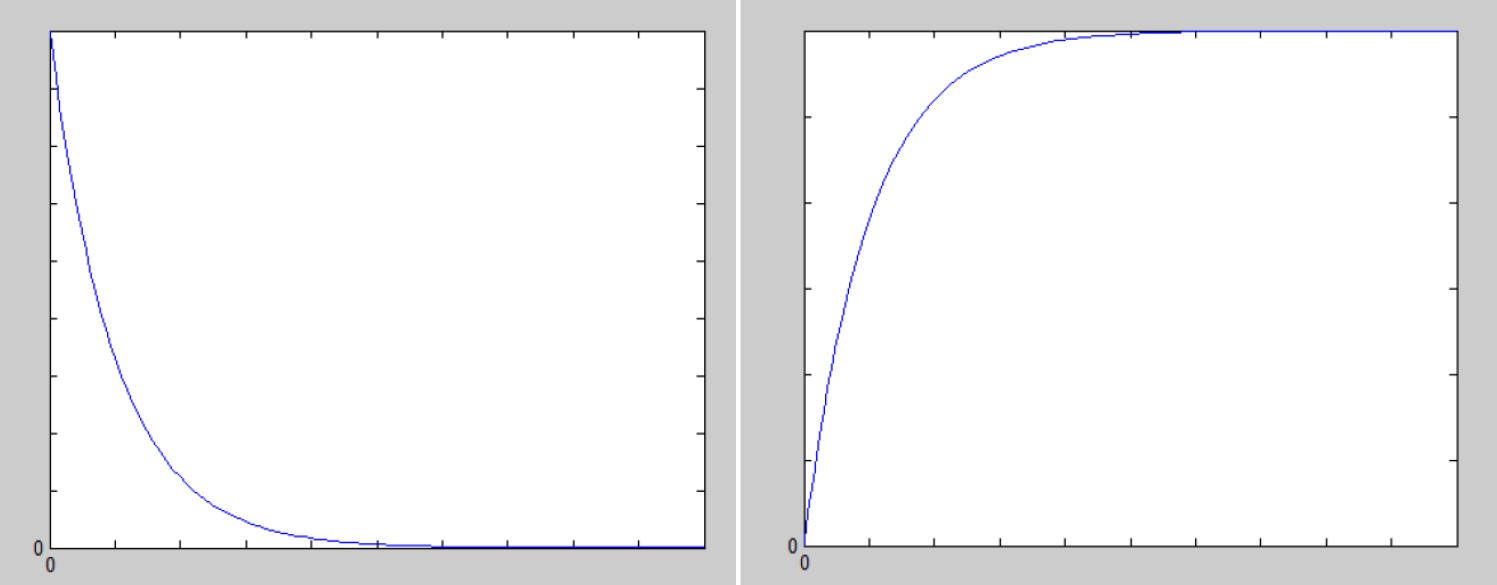
\includegraphics[scale=0.4]{TP5/RC.PNG}
\end{center}

%QUESTION 1.1.
\Question
{
%question
\textit{Identifiez l'élément du schéma (source(s), capacité, resistance(s)) auquel se rapportent ces deux graphes.\\
Identifiez la grandeur (tension(s) ou courant(s)) présente sur l'ordonnée pour chaque courbe.}
}
{
\textbf{Elément:} La capacité\\

\textbf{A droite:}\\
Il s'agit de la tension aux bornes du condensateur $v_C(t)$.\\

Vérification numérique après résolution de la Question 1.4.:\\
$v_C(t)=\frac{5E}{2}(1-\exp{(-\frac{t}{C(R+r/4)})})=50(1-\exp{(-\frac{t}{0,2})}) [V]$ avec une tension initiale $v_C(0-)=v_C(0+)=0V$ et une tension de régime $v_C(\infty)=50V$\\


\textbf{A gauche:}\\
Il s'agit de l'intensité de courant $i(t)$ traversant le condensateur.\\

Vérification numérique après résolution de la Question 1.4.:\\
$i(t)=\frac{10E}{4R+r}exp{(-\frac{t}{C(R+r/4)})}=25 exp{(-\frac{t}{0,2})} [A]$ avec $i(0-)=0A$, $i(0+)=25A$ et $i(\infty)=0A$.
}


%QUESTION 1.2.
\Question
{
%question
\textit{Sur base de ce graphique, déterminer la valeur de la constante de temps $\tau$ du circuit.}
}
{
La constante de temps $\tau$ est par définition le temps nécessaire à la tension aux bornes du condensateur pour atteindre $63\%$ de sa valeur de régime:
$$v_C(\tau)=v_C(\infty)(1-\exp{(-1}))\cong 0,63v_C(\infty)$$

Graphiquement, il suffit de tracer une ligne horizontale passant par $0,63\times 50=31,5V$.\\ L'intersection avec le graphique de $v_C(t)$ donne $\tau=0,2s$.\\

Il était également possible d'utiliser la méthode graphique de la tangente à l'origine (moins précis).

Vérification numérique après résolution:
$$\tau=C(R+\frac{r}{4})=0,1.(1+\frac{4}{4})=0,2s$$
}

%QUESTION 1.3.
\Question
{
%question
\textit{Déterminez les paramètres $R_{th}$ et $V_{th}$ de l'équivalent de Thévenin du circuit vu aux bornes du condensateur.}
}
{
\fbox{$R_{th}$}\\
Pour trouver la résistance équivalente de Thévenin, il faut court-circuiter les sources du circuit. (1 point)

\begin{center}
\begin{circuitikz}[scale=0.6] \draw
(0,0)   node [ground] {}
		to	 [short]	(0,2)
		to	 [R, l=$r$]							(0,4)--(2,4)
(2,0)	to	 [short]	(2,2)
		to	 [R, l=$r$]							(2,4)--(4,4)
(4,0)	to	 [short]	(4,2)
		to	 [R, l=$r$]							(4,4)--(6,4)
(6,0)	to	 [short]	(6,2)
		to	 [R, l=$r$]							(6,4)
		to	 [short]					(8,4)
		to   [R, l=$R$]							(8,2)
		to   [open, l=$R_{th}$]							(8,0)--(0,0)	
;
\end{circuitikz}
\end{center}

Par les propriétés de la mise en parallèle et de la mise en série de résistances (2 points):
$$R_{th}=R+(r//r//r//r)=R+\frac{r}{4}$$

\fbox{$V_{th}$}\\
Pour trouver la tension équivalente de Thévenin, on doit résoudre le circuit à vide (remplacer le condensateur par un circuit ouvert). Le courant passant dans la branche de droite est alors nul et il n'y a pas de chute de potentiel dans la résistance $R$ ($V_R=Ri=0$).  (1 point)\\

\begin{center}
\begin{circuitikz}[scale=0.8] \draw
(0,0)   node [ground] {}
		to	 [american voltage source, v=$E$,  i^>=$i_1$, invert]	(0,2)
		to	 [R, l=$r$]							(0,4)--(2,4)
(2,0)	to	 [american voltage source, v=$2E$, i^>=$i_2$, invert]	(2,2)
		to	 [R, l=$r$]							(2,4)--(4,4)
(4,0)	to	 [american voltage source, v=$3E$, i^>=$i_3$, invert]	(4,2)
		to	 [R, l=$r$]							(4,4)--(6,4)
(6,0)	to	 [american voltage source, v=$4E$, i^>=$i_4$, invert]	(6,2)
		to	 [R, l=$r$]							(6,4)
		to	 [short]							(8,4)
		to   [R, l=$R$]							(8,2)
		to   [open, v^=$V_{th}$]					(8,0)
		to	 [short, i=$i$]						(6,0)--(0,0)	
;
\end{circuitikz}
\end{center}


\textbf{Résolution 1 - Lois de Kirchhoff:} (1 point méthode + 3 points résolution)

Soit $i_{k}(t)$ le courant passant dans la $k\up{ième}$ branche (de gauche à droite).

La mise en parallèle des cinq branches nous permet d'égaler les tensions:
$$V_{th}=E-ri_{1}=2E-ri_{2}=3E-ri_{3}=4E-ri_{4}$$

Par la loi des noeuds, on a donc:\\
$i(t)=\sum_{k=1}^{4} (i_{k}(t))=0$\\
$\Leftrightarrow i_{1}+i_{1}+\frac{E}{r}+i_{1}+\frac{2E}{r}+i_{1}+\frac{3E}{r}=4i_{1}+6\frac{E}{r}=0$\\
$\Leftrightarrow i_{1}=-\frac{3}{2} \frac{E}{r}$

Et donc finalement:
$$V_{th}=E-ri_{1}=\frac{5}{2} E$$


\textbf{Résolution 2 - Théorème de superposition:} (1 point méthode + 3 points résolution)\\

Soit $E_i (i=1,2,3,4)$ les 4 sources et $V_{th_i}$ les contributions de chacune d'elle à la tension de Thévenin.

On annule donc toutes les sources sauf $E_i$ pour les 4 cas $(i=1,2,3,4)$, on calcule chacune des contributions puis on les somme pour avoir $V_{th}$.

\textit{Remarque:}\\
Beaucoup d'entre vous ne se sont pas rendu compte que les 4 branches contenant les sources sont en parallèle et donc permutables. Cela engendre le même développement analytique pour chacune des branches!\\

En utilisant la propriété de mise en parallèle des 3 résistances $r$ des 3 branches sans source, on obtient le diviseur résistif respectant l'équation:\\
$$V_{th_i}=\frac{\frac{r}{3}}{\frac{r}{3}+r}*E_i=\frac{E_i}{4}$$

Et donc:\\
$$V_{th}=\sum_{i=1}^{4} V_{th_i}=\sum_{i=1}^{4} \frac{E_i}{4}=\frac{E_1+E_2+E_3+E_4}{4}=\frac{E+2E+3E+4E}{4}=\frac{5}{2} E$$

Le circuit complet (équivalent de Thévenin + capa) peut donc être représenté par un circuit RC comme suit:

\begin{center}
\begin{circuitikz} \draw
(0,0)   node [ground] {}
		to	 [american voltage source, v=$2.5V$,  i^>=$i$, invert]	(0,2)
		to	 [R, l=$R+\frac{r}{4}$]	(2,2)
		to	 [C, v^<=$V_C$] (2,0)
		to	 [short, i=$i$] (0,0)
;
\end{circuitikz}
\end{center}


}

\Question
{
%question
\textit{Maintenant, résolvez le circuit analytiquement (méthode au choix) afin de déterminer la tension $v_C(t)$ aux bornes du condensateur ainsi que l'intensité de courant $i(t)$ le traversant pour tout temps $t\geq0$.}
}
{
\textit{Remarque:}\\
Vous avez été nombreux a utiliser les phaseurs pour résoudre ce circuit. Pour rappel, les phaseurs dévoilent toute leur utilité lorsqu'on est dans une situation en régime permanent avec sollicitation(s) sinusoïdale(s). Ici, on cherche à trouver les solutions de régime permanent mais aussi du transitoire! De plus, les sources de tension ici sont en continu. On a donc un $\omega=0 rad/s$!\\

\underline{\textbf{METHODE 1 (utiliser l'équivalent de Thévenin de la question précédente)}}

L'équivalent de Thévenin trouvé précédemment nous donne l'équation de maille:  (1 point)
$$V_{th}=R_{th}i+v_C \Leftrightarrow \frac{5}{2}E=(R+\frac{r}{4})i+v_C$$

La loi du condensateur étant $i(t)=C\frac{dv_C(t)}{dt}$ (1 point), on obtient l'équation différentielle du premier ordre:
$$\frac{4R+r}{4}C \frac{dv_C}{dt}+v_C=\frac{5E}{2}$$

Solution générale de l'équation homogène $\frac{4R+r}{4}C\frac{dv_C}{dt}+v_C=0$: (2 points)
$$\frac{dv_C}{v_C}=-\frac{1}{C(R+\frac{r}{4})}dt$$

Puis on intègre:\\
$$\int \frac{dv_C}{v_C}=-\frac{1}{C(R+\frac{r}{4})}\int dt \Leftrightarrow ln(v_C)=-\frac{1}{C(R+\frac{r}{4})}t+constante$$
$$\Leftrightarrow v_{C_g}(t)=K \exp{(-\frac{t}{C(R+\frac{r}{4})})}$$

Solution particulière de l'équation non-homogène $\frac{4R+r}{4}C\frac{dv_c}{dt}+v_c=\frac{5E}{2}$:  (2 points)\\
Il s'agit de la solution de régime, donc $\frac{dv_c}{dt}=0$ (circuit ouvert) et:
$$v_{C_p}=\frac{5E}{2}$$

Solution générale de l'équation non-homogène:
$$v_C(t)= v_{C_g}(t)+v_{C_p}=K \exp{(-\frac{t}{C(R+\frac{r}{4})})}+\frac{5E}{2}$$

La charge initiale nulle et la loi de continuité en tension d'un condensateur nous donnent (1 point):
$$v_C(0+)=v_C(0-)=0$$
Ce qui permet de déterminer la constante d'intégration K:
$$v_C(0)=K+\frac{5E}{2}=0 \Leftrightarrow K=-\frac{5E}{2}$$

\textit{Réponses finales:} (1 point)

\begin{center}
$\Rightarrow$ \fbox{$v_C(t)=\frac{5E}{2}(1-\exp{(-\frac{t}{C(R+\frac{r}{4})})})$}
\end{center}

Pour le courant, on a $i(t)=C\frac{dv_c(t)}{dt}$:
\begin{center}
$\Rightarrow$ \fbox{$i(t)=\frac{10E}{4R+r}exp{(-\frac{t}{C(R+\frac{r}{4})})}$}    
\end{center}

\underline{\textbf{METHODE 2 (en cas d'échec à la question précédente)}}\\
\begin{center}
\begin{circuitikz}[scale=0.8] \draw
(0,0)   node [ground] {}
		to	 [american voltage source, v=$E$,  i^>=$i_1$, invert]	(0,2)
		to	 [R, l=$r$]							(0,4)--(2,4)
(2,0)	to	 [american voltage source, v=$2E$, i^>=$i_2$, invert]	(2,2)
		to	 [R, l=$r$]							(2,4)--(4,4)
(4,0)	to	 [american voltage source, v=$3E$, i^>=$i_3$, invert]	(4,2)
		to	 [R, l=$r$]							(4,4)--(6,4)
(6,0)	to	 [american voltage source, v=$4E$, i^>=$i_4$, invert]	(6,2)
		to	 [R, l=$r$]							(6,4)
		to	 [closing switch]							(8,4)
		to   [R, l=$R$]							(8,2)
		to   [C, v^<=$V_{th}$]					(8,0)
		to	 [short, i=$i$]						(6,0)--(0,0)	
;
\end{circuitikz}
\end{center}
Soit $i_{k}(t)$ le courant passant dans la $k\up{ième}$ branche (de gauche à droite) tel que le courant passant dans le condensateur $i(t)=\sum_{k=1}^{4} (i_{k}(t))$ par la loi des noeuds.\\

La mise en parallèle des cinq branches nous permet d'égaler les tensions:
$$E-ri_{1}=2E-ri_{2}=3E-ri_{3}=4E-ri_{4}=v_c+Ri$$
Et donc, on a:
$$i=i_{1}+i_{2}+i_{3}+i_{4}=i_{1}+i_{1}+\frac{E}{r}+i_{1}+\frac{2E}{r}+i_{1}+\frac{3E}{r}=4i_{1}+6\frac{E}{r}$$
En inversant l'équation:
$$i_{1}=\frac{i}{4}-\frac{3}{2}\frac{E}{r}$$

De plus:
$$v_C+Ri=E-ri_{1} \quad\text{et}\quad i(t)=C\frac{dv_C(t)}{dt} $$

Donc:
$$v_C+Ri=E-r\frac{i}{4}-\frac{3}{2}E$$
$$\Leftrightarrow \frac{4R+r}{4}C \frac{dv_C}{dt}+v_C=\frac{5E}{2}$$

Et on retombe bien sur l'équation différentielle vue précédemment.
}

%QUESTION 2.3.
\subsection{Question de l'Examen de Janvier 2013}

\begin{center}
\begin{circuitikz} [scale=0.8] \draw
(0,0)   node [ground] {}
		to	 [sinusoidal voltage source, v=$E$]	(0,3)
		to	 [R, l=$R_1$] 	(3,3)
		to	 [R, l=$R_2$]	(3,0)
		to	 [L, l=$L_1$]	(0,0)
(3,3)--(5,3)
		to	 [R, l=$R_3$]	(5,0)--(3,0)
;
\end{circuitikz}
\end{center}

Soit le circuit représenté ci-dessus dont les paramètres sont:
\begin{itemize}
\item $\underline{E}=5V\times e^{j\phi}$ (on considère donc le courant comme référence, c'est-à-dire $\underline{I}=I\times e^{j0^o}$)
\item $R_1=3\Omega$, $R_2=5\Omega$ et $R_3=1,25\Omega$
\item $L_1=9,55mH=\frac{30}{\pi}mH$
\item $f=50Hz$
\end{itemize}

\vspace{5mm}
\Question
{%Q
\textit{Que vaut le module du courant circulant dans $L_1$?}
}
{%A
$$Z_{tot}= R_1+R_2//R_3+j\omega L_1=R_1+\frac{R_2 R_3}{R_2+R_3}+j\omega L_1$$
$$=3+\frac{5\times1,25}{5+1,25}+j2\pi 50\times \frac{30}{\pi}=4+j3=\sqrt{4^2+3^2}\times e^{arctan(\frac{3}{4})}=5\times e^{j36,9^o}$$
}

\Question
{%Q
\textit{Que vaut le déphasage $\phi$ entre la tension $\underline{E}$ et le courant débité par la source?}
}
{%A
Comme on a trouvé:
$$\underline{I}=\frac{\underline{E}}{Z_{tot}}=1Ae^{j(\phi-36,9^o)}$$
On en déduit que $\phi=36,9^o$ tel que:
$$\underline{I}=I\times e^{j0^o}=1A$$
Autre méthode:
$$Z_{tot}=\frac{\underline{E}}{\underline{I}} \Rightarrow \phi=\phi_E-\phi_I=Arg(Z_{tot})=arctan(\frac{\omega L_1}{R_1+\frac{R_2 R_3}{R_2+R_3}})=arctan(\frac{3}{4})=36,9^o$$
}

\Question
{%Q
\textit{Calculer les phaseurs de chacune dans 5 tensions suivantes: $\underline{E}$, $\underline{V}_{R_1}$, $\underline{V}_{R_2}$, $\underline{V}_{R_3}$ et $\underline{V}_{L_1}$?}
}
{%A
$$\underline{E}=Z_{tot}\underline{I}=5V\times e^{36,9^o}$$
$$\underline{V}_{R_1}=R_1\underline{I}=3V$$
$$\underline{V}_{R_2}=\underline{V}_{R_3}=\frac{R_2 R_3}{R_2+R_3}\underline{I}=4V$$
$$\underline{V}_{L_1}=j\omega L_1 \underline{I}=j3=3V\times e^{j 90^o}$$

}

\Question
{%Q
\textit{Dessiner le diagramme des phaseurs des 5 tensions présentés dans le circuit en utilisant la tension $\underline{V}_{R_2}$ comme référence.}\\
\textit{Proposer un diagramme cohérent si vous n'avez pas su calculer les différentes tensions.}\\

\begin{center}
\begin{tikzpicture}
\draw (0,0) grid[step=0.5] (10,10);
\end{tikzpicture}
\end{center}
}
{%A
\begin{center}
\begin{tikzpicture}
\draw (0,0) grid[step=1] (10,10);
\draw[-stealth, blue] (0,3)--(6,3) node[midway, below]{$\underline{V}_{R_1}$};
\draw[-stealth, blue] (6,3)--(8,3) node[midway, above]{$\underline{V}_{R_2}=\underline{V}_{R_3}$};
\draw[-stealth, blue] (8,3)--(8,9) node[midway, below]{$\underline{V}_{L_1}$};
\draw[-stealth, blue] (0,3)--(8,9) node[midway, below]{$\underline{E}$};
\end{tikzpicture}
\end{center}
}

\subsection{Question de l'Examen d'Août 2014}

\begin{center}
\begin{circuitikz} \draw
(0,0)   node [ground] {}
		to[sinusoidal voltage source, v=$V_i$] (0,3)
		to[R, l=$R$]						 (4,3)
		to[L, l=$L$]						 (4,0)
		to[R, l=$R_e$]						 (0,0)
(1,3) node[circ]{A}
(1,0) node[circ]{B}
(3,0) node[circ]{C}
;
\end{circuitikz}
\end{center}

Avec $R=2\Omega$, $R_e=1\Omega$, $L=5,5mH$ et $f=50Hz$.
\Question
{%Q
\textit{En utilisant la tension $\underline{V}_{CB}=1V*e^{j0^o}$ comme référence, donner l'expression des phaseurs $\underline{V}_{AB}$ et $\underline{V}_{AC}$.}
}
{%A
On trouve \underline{I} grâce à $\underline{V}_{CB}$ qui est donné: $$\underline{I}=\frac{\underline{V}_{CB}}{R_e}=1A*e^{j0^o}$$
Connaissant le courant et les impédances, par la loi d'Ohm:
$$\underline{V}_{AB}=(R+R_e+j\omega L)\underline{I}=(R+R_e+j\omega L)\frac{\underline{V}_{CB}}{R_e}=3+j2\pi 50*5,5*10^{-3}=3+j\sqrt{3}$$
$$\underline{V}_{AC}=(R+j\omega L)\frac{\underline{V}_{CB}}{R_e}=2+j2\pi 50*5,5*10^{-3}=2+j\sqrt{3}$$
}


\subsection{Question 7}
\begin{center}
\begin{circuitikz} \draw
(1,0)   to[R, l=$R_3$] 						(-1,2)
		to[R, l=$R_4$]    					(1,4)
		to[R, l=$R_1$]	            	    (3,2)
		to[R, l=$R_2$]	   					(1,0) -- (6,0)
(3,2) -- (6,2)
(1,4) -- (1,5)
		to[sinusoidal voltage source, v=$E$](5,5) -- (5,2)
node[circ] (B) at (6,0) {B}
node[circ] (A) at (6,2) {A}
(B) to [open, v_=$\underline{V}_{Th}?\ Z_{Th}?$] (A)
;
\end{circuitikz}
\end{center}

Soit le circuit représenté ci-dessus dont deux nœuds ont été nommés A et B pour la clarté de l’énoncé et dont les paramètres sont donnés ci-dessous:
\begin{itemize}
	\item $\underline{E}=6V.e^{j0^{\circ}}$
	\item $R_1=5\Omega, R_2=4\Omega, R_3=6\Omega, R_4=10\Omega$
\end{itemize}
\vspace{5mm}
%QUESTION 1.1.
\Question
{
\textit{Calculer l'équivalent de Thévenin vu par l’accès AB.}
}
{%answer
La source $ \underline{V}_{Th} $ se calcule en trouvant la tension à l'accès AB à vide.\\
Il suffit de calculer le diviseur d'impédance:
$$ V_{AB}=V_{Th}=\frac{R_2}{R_2+R_3+R_4}V_i=\frac{6}{5}V $$

%$$ \fbox{V_{Th} = \frac{6}{5}V = 1,2V} $$
\begin{equation*}
	V_{Th}
\end{equation*}

$Z_{Th}$ se calcule en court-circuitant la source. On a:
$$Z_{Th}=R_2//(R_3+R_4)=\frac{1}{\frac{1}{R_2}+\frac{A}{R_3+R_4}}=\frac{1}{\frac{1}{4}+\frac{1}{16}}=\frac{16}{5}$$
$$ Z_{Th} = \frac{16}{5} = 3,2V $$
}


%QUESTION 1.2.

\begin{center}
\begin{circuitikz} \draw
(1,0)   to[R, l=$R_3$] 						(-1,2)
		to[R, l=$R_4$]    					(1,4)
		to[R, l=$R_1$]	            	    (3,2)
		to[R, l=$R_2$]	   					(1,0)
(3,2) -- (6,2)
(1,4) -- (1,5)
		to[sinusoidal voltage source, v=$e(t)$, i_>=$i(t)$](4,5) 
		
(4.5,5) node[spdt] (Sw) { }
(Sw.in) node[ left ] {}
(Sw.out 1) node[right] {C} -- (6,5.3) -- (6,2)
(Sw.out 2) node[right] {D} to[L, l=$L_1$]       (5.1,2)
;
\end{circuitikz}
\end{center}

Soit le circuit ci-dessus repris de la question 1, pour lequel: $L_1=6,37mH=\frac{20}{\pi}mH$ et  $f=50Hz$.
\begin{itemize}
	\item Avant l'instant $t_1=0$, la source $e(t)=0V$ et l'interrupteur est connecté à la borne C.
	\item Au temps $t_1=0$, on active la source $e(t)=6V \sin(\omega t)$ et l'interrupteur reste connecté à C.
	\item Au temps $t_2=100ms$, l'interrupteur passe (de manière instantanée) de la borne C à la borne D.
\end{itemize}
\vspace{3mm}

\Question
{
\textit{Calculer le courant $i(t)$ délivré par la source $e(t)$ pour tout temps $t$.}
}
{%answer
\begin{enumerate}
\item de $t_1$ à $t_2$, il n'y a que des résistances, donc pas de transitoire. On calcule la résistance équivalente du montage:
$$R=R_1//(R_2+R_3+R_4)=4\Omega$$
Et donc,
$$i(t\in[t_1;t_2])=\frac{3}{2}\sin(\omega t)$$
\item en $t\geq t_2$. On devra connaitre les conditions de $i(t_2)$. Facile car $\sin(\omega t_2)=0$.
$$e(t)=Ri(t)+L\frac{di}{dt} \Rightarrow i(t) = Ae^{-\frac{R}{L}t}+i_P$$
$$\underline{I}_P=\frac{\underline{E}}{R+j\omega L}\Rightarrow i_P(t)=\frac{E}{\sqrt{R^2+(\omega L)^2}} \sin(\omega t - \theta)$$
avec $$\theta=arctan(\frac{\omega L}{R})$$
%\begin{itemize}
%	\item $Z=R4+2j\Omega$\\
%	$i_R(t)=\frac{6}{4+2j}\sin(\omega t)=(1,2-0,6)\sin(\omega t)$ pour $t\in[t_2;t_\infty]$
%	\item valeur en transitoire + régime\\
%	$i(t)=\frac{6}{\sqrt{4^2+2^2}}[\sin(\omega t)+26,6^{\circ}+\sin(26,6^{\circ})\exp^{2t})]$
%\end{itemize}
Avec les conditions initiales, on obtient:
$$i(t) = \frac{E}{\sqrt{R^2+(\omega L)^2}}(sin(\omega t-\theta)-e^{-\frac{R}{L}t}sin(\theta))$$
\end{enumerate}

En conclusion:
$$i(t)=1,5A\sin(\omega t)\ pour\ t\in[0;100ms]$$
$$i(t)=2\sqrt{5}A[\sin(\omega t-26,6^{circ})+\sin(26,6^{circ})e^{-2t}])\ pour\ t\in[100ms;\infty]$$
}

\subsection{Question de l'Examen d'Août 2014}
\begin{center}
\begin{circuitikz} \draw
(0,0)   to[american voltage source, l=$e(t)$, i^>=$i(t)$, invert] 	(0,5)
		to[L, l=$L_1$]    				(3,5)
		to[L, l=$L_2$]	                (3,2.5)
		to[R, l=$R$]	   				(3,0) -- (0,0)
(3,5) -- (5,5)
to[american current source, l_=$i_S(t)$]  (5,0) -- (3,0)			
node (A) at (5.5,1) {}
node (B) at (5.5,4) {}
(A) to [open, v_=$v(t)$] (B)
%node[circ] (C) at (0.8,4.8) {}
%node[circ] (D) at (2.8,3) {}
%(D) to [open, v^=$M$] (C)
%(C) to [open, v=$ $] (D)
;
\end{circuitikz}
\end{center}

\vspace{-5mm}
Soit le circuit représenté ci-dessus comportant:\\
\begin{itemize}
	\item Une source de tension $e(t)=E_{0}+E_{1}\cos(\omega_1 t)$\\
	avec $E_0=3V$, $E_1=5V$ et $\omega_1=1000 rad/s$;
	\item Une source de courant $i_{s}(t)=I_{s}\sin(\omega_2 t+\phi)$\\
	avec $I_S=1A$, $\omega_2=2000 rad/s$ et $\phi=30^{\circ}$;
	\item $R=1\Omega$, $L_1=2mH$, $L_2=1mH$.
\end{itemize}
\vspace{5mm}

On cherche à déterminer la tension $v(t)$ en régime établi.

%QUESTION 2.1.
\Question
{
%question
\textit{Quelles vont être les étapes de votre démarche afin de résoudre ce circuit et de trouver la tension $v(t)$ en régime établi?\\
Détaillez votre démarche sans recourir aux équations. }
}
{
\begin{itemize}
	\item \textbf{Définir les courants et tensions} sur le schéma \textbf{en respectant les conventions} générateur/récepteur
	\item Utiliser le \textbf{principe de superposition}: \textbf{pour chacun des 3 cas} ($\omega=0$, $\omega=\omega_1$ et $\omega=\omega_2$):
	\begin{itemize}
		\item \textbf{Simplification du schéma}\\
			Inductance = court-circuit en continu, source de tension nulle = court-circuit, source de courant nulle = circuit ouvert.
		\item \textbf{Exprimer les grandeurs en phaseurs} car nous cherchons la tension de régime
		\item \textbf{Equations de Kirchhoff}\\
			Loi des mailles: La somme algébrique des tensions aux bornes des branches constituant une maille est nulle.\\
			Loi des noeuds: La somme algébrique des courants quittant un noeud est nulle.
		\item \textbf{Résolution de l'équation/du système d'équations} par les méthodes algébriques classiques.
		\item Exprimer le résultat \textbf{dans le domaine temporel}.
	\end{itemize}
	\item Effectuer la \textbf{superposition}, c'est-à-dire sommer les 3 réponses temporelles.
\end{itemize}
}


%QUESTION 2.2.
\Question
{
\textit{Déterminer la tension $v(t)$ en régime établi.\\
\textbf{Pour vos calculs}: Ne pas déterminer les valeurs des arctangentes (laisser sous la forme $\arctan{x}$) et utiliser si besoin les approximations suivantes: $\sqrt{185} \approx 14$ et $\frac{4}{37} \approx 0,1$.}
}
{%answer
Puisque le circuit comporte 3 sources de pulsations différentes, l'utilisation du théorème de superposition est nécessaire.\\

\fbox{$\omega=0rad/s$}\\
En régime continu, les inductances se comportent comme des courts-circuits. En ne gardant que la source de tension $E_0$ et en annulant les deux autres sources, on obtient en phaseurs: $v_0=RI=E_0=3V$
\begin{center}
\begin{circuitikz} \draw
(0,0)   to[american voltage source, l=$e(t)$, i^>=$i(t)$, invert] 	(0,3)
		--    				(3,3)
		
		to[R, l=$R$]	   				(3,0) -- (0,0)
(3,3) -- (5,3)
to[open]  (5,0) -- (3,0)			
node (A) at (5.5,0) {}
node (B) at (5.5,3) {}
(A) to [open, v_=$v_0(t)$] (B)
%node[circ] (C) at (0.8,4.8) {}
%node[circ] (D) at (2.8,3) {}
%(D) to [open, v^=$M$] (C)
%(C) to [open, v=$ $] (D)
;
\end{circuitikz}
\end{center}

\fbox{$\omega=\omega_1=1000rad/s$}\\
En ne gardant que la source de tension $E_{1}\cos(\omega_1 t)$ et en annulant les deux autres sources, on obtient le circuit suivant:
\vspace{-5mm}
\begin{center}
\begin{circuitikz} \draw
(0,0)   to[american voltage source, l=$E_1 \cos(\omega_1 t)$, i^>=$i(t)$, invert] 	(0,5)
		to[L, l=$L_1$]    				(3,5)
		to[L, l=$L_2$]	                (3,2.5)
		to[R, l=$R$]	   				(3,0) -- (0,0)
(3,5) -- (5,5)
to[open]  (5,0) -- (3,0)			
node (A) at (5.5,1) {}
node (B) at (5.5,4) {}
(A) to [open, v_=$v_1(t)$] (B)
%node[circ] (C) at (0.8,4.8) {}
%node[circ] (D) at (2.8,3) {}
%(D) to [open, v^=$M$] (C)
%(C) to [open, v=$ $] (D)
;
\end{circuitikz}
\end{center}

Ce diviseur impédant donne l'expression suivante:\\
$\underline{V}_1=\frac{R+j\omega_1 L_2}{R+j\omega_1 (L_1+L_2)}\underline{E}_1$\\
$\underline{V}_1=\frac{1+j}{1+3j}\underline{E}_1=\frac{4-2j}{10}\underline{E}_1=\frac{2-j}{5}\underline{E}_1=\frac{\sqrt{5}}{5}\exp(-j \arctan \frac{1}{2}) E_1 \exp (j0^{\circ})=\sqrt{5}\exp(-j \arctan \frac{1}{2})$\\

%$\underline{E_1}=(R+j\omega_1 (L_1+L_2-2M))  \underline{I}$\\
%$\underline{V_1}=(R+j\omega_1(L_2-M)) \underline{I}$\\
%$\Leftrightarrow$\\
%$\underline{I}=\frac{\underline{E_1}}{R+j\omega_1 (L_1+L_2-2M)} $\\
%$\underline{V_1}=\frac{R+j\omega_1(L_2-M)}{R+j\omega_1 (L_1+L_2-2M)}\underline{E_1}=\frac{1+j}{1+2j}\underline{E_1}=\frac{3-j}{5}\underline{E_1}\\
%=\frac{\sqrt{10}}{5}\exp{(-j \arctan{\frac{1}{3}})}E_1\exp{(j0^{\circ})}=\frac{\sqrt{10}}{5}5\exp{(-j \arctan{\frac{1}{3}})}$\\

Et donc, dans le domaine temporel:\\
$v_1(t)=\sqrt{5}cos(1000t-\arctan{\frac{1}{2}})$

\fbox{$\omega=\omega_2=2000rad/s$}\\
En ne gardant que la source de courant $i_{s}(t)=I_{s}\sin(\omega_2 t+\phi)$ et en annulant les deux autres sources, on obtient le système de trois équations à trois inconnues suivant (2 équations de maille et 1 équation de noeud):\\
\shorthandoff{:!}
\begin{center}
\begin{circuitikz} \draw
(0,0)   to[short , i_=$i_1(t)$] 	(0,5)
		to[L, l=$L_1$, v<=$v_{L_1}$]    				(3,5)
		to[L, l=$L_2$, v>=$v_{L_2}$]	                (3,2.5)
		to[R, l=$R$, v>=$v_R$, i<_=$i_2(t)$]	   				(3,0) -- (0,0)
(3,5) -- (5,5)
to[american current source, l_=$i_S(t)$]  (5,0) -- (3,0)			
node (A) at (5.5,1) {}
node (B) at (5.5,4) {}
(B) to [open, v^<=$v_2(t)$] (A)
%node[circ] (C) at (0.8,4.8) {}
%node[circ] (D) at (2.8,3) {}
%(D) to [open, v^=$M$] (C)
%(C) to [open, v=$ $] (D)
;
\end{circuitikz}
\end{center}
\shorthandon{:!}
%\begin{center}
%	\includegraphics[width=8cm]{circuit_mutuelle_omega2.png}
%\end{center}


    $$\underline{V}_{L_1} = \underline{V}_{R}+\underline{V}_{L_2}$$
    $$\underline{V}_2 = -(\underline{V}_{R}+\underline{V}_{L_2})$$
    $$\underline{I_s} = \underline{I_1}+\underline{I_2}$$


Donc, $\underline{V}_2=-\underline{V}_{L_1}=-j \omega_2 L_1 \underline{I}_1$ et il nous suffit de trouver $\underline{I_1}$ en fonction de $\underline{I}_S$.\\

$$\underline{V}_{L_1} = \underline{V}_{R}+\underline{V}_{L_2}$$
$$\Rightarrow j \omega_2 L_1 \underline{I}_1=(R+j\omega_2 L_2) \underline{I}_2=(R+j\omega_2 L_2) (\underline{I}_S-\underline{I}_1)$$
$$\Rightarrow (R+j \omega_2 (L_1+L_2)) \underline{I}_1=(R+j\omega_2 L_2) \underline{I}_S$$
$$\Rightarrow \underline{I}_1=\frac{R+j\omega_2 L_2}{R+j \omega_2 (L_1+L_2)} \underline{I}_S$$
$$\Rightarrow \underline{V}_2=-\underline{V}_{L_1}=-j \omega_2 L_1 \underline{I}_1=-j \omega_2 L_1\frac{R+j\omega_2 L_2}{R+j \omega_2 (L_1+L_2)} \underline{I}_S$$

Numériquement:\\
$$\underline{V}_2=-4j \frac{1+2j}{1+6j}\underline{I}_S=4\frac{(2-j)}{1+6j}\underline{I}_S=4\frac{(2-j)(1-6j)}{1^2+6^2}\underline{I}_S=-4\frac{4+13j}{37}\underline{I}_S$$

Avec le phaseur $\underline{I_s}=I_s e^{j\phi}=1A e^{j30^{\circ}}$, on obtient:
$$\underline{V_2}=-\frac{4}{37}\sqrt{4^2+13^2}e^{(j(30^{\circ}+\arctan{\frac{13}{4}))}}=-\frac{4}{37}\sqrt{185}e^{(j(30^{\circ}+\arctan{3,25})} \\ \approx -1,4 e^{(j(30^{\circ}+\arctan{3,25})}$$

Et donc, dans le domaine temporel:
$$v_2(t)=-1,4 \sin(2000t+30^{\circ}+\arctan{3,25})$$

Par le théorème de superposition, on a la solution finale $v(t)=v_0+v_1(t)+v_2(t)$:
$$ v(t)=3+\sqrt{5}cos(1000t-\arctan{\frac{1}{2}})-1,4 \sin(2000t+30^{\circ}+\arctan{3,25}) $$
}


\end{document}